\documentclass[11pt]{article}

% ---------- Layout ----------
\usepackage[a4paper,margin=2.2cm]{geometry}
\usepackage[T1]{fontenc}
\usepackage[utf8]{inputenc}
\usepackage{lmodern}
\usepackage{parskip}
\usepackage{fancyhdr}
\usepackage{titlesec}
\usepackage{enumitem}
\usepackage{xcolor}
\usepackage{booktabs}
\usepackage{longtable}
\usepackage{tabularx}
\usepackage{framed}
\usepackage{amssymb}
\usepackage{listings}
\usepackage{caption}
\usepackage{graphicx}
\usepackage{float}
\usepackage{hyperref}
\usepackage{tikz}
\usetikzlibrary{arrows.meta,positioning,shapes.geometric,fit,backgrounds,calc,decorations.pathreplacing}

% ---------- Colors ----------
\definecolor{stagefill}{RGB}{232,242,252}
\definecolor{stageline}{RGB}{60,110,180}
\definecolor{warnfill}{RGB}{253,237,224}
\definecolor{warnline}{RGB}{200,120,30}
\definecolor{okfill}{RGB}{228,246,232}
\definecolor{okline}{RGB}{40,140,70}
\definecolor{badfill}{RGB}{252,230,230}
\definecolor{badline}{RGB}{190,50,50}
\definecolor{codebg}{RGB}{245,245,248}
\definecolor{linknote}{RGB}{90,60,140}
\definecolor{stage2fill}{RGB}{255,244,230}
\definecolor{stage2line}{RGB}{190,120,20}
\definecolor{flashline}{RGB}{185,121,31}
\definecolor{bucketline}{RGB}{70,87,140}

% ---------- Section styling ----------
\titleformat{\section}{\normalfont\Large\bfseries\color{stageline}}{\thesection}{0.6em}{}
\titleformat{\subsection}{\normalfont\large\bfseries}{\thesubsection}{0.6em}{}
\titleformat{\subsubsection}{\normalfont\bfseries}{\thesubsubsection}{0.6em}{}

% ---------- Header/Footer ----------
\pagestyle{fancy}
\fancyhf{}
\renewcommand{\headrulewidth}{0.4pt}
\fancyhead[L]{\small The simple-mde-gmn Pipeline}
\fancyhead[R]{\small\leftmark}
\fancyfoot[C]{\thepage}

% ---------- Step-list environments ----------
\newlist{steps}{enumerate}{2}
\setlist[steps,1]{label=\textbf{Step \arabic*:},leftmargin=1.3em,itemindent=1.4em,itemsep=5pt,topsep=5pt,parsep=2pt}
\setlist[steps,2]{label=\textbf{Step \arabic{stepsi}.\arabic*:},leftmargin=1.3em,itemindent=2.0em,itemsep=3pt,topsep=3pt,parsep=1pt}

% ---------- Code listing style ----------
\lstset{
  basicstyle=\ttfamily\small,
  backgroundcolor=\color{codebg},
  frame=single,
  rulecolor=\color{gray!40},
  breaklines=true,
  columns=fullflexible,
  xleftmargin=4pt, xrightmargin=4pt,
  aboveskip=6pt, belowskip=6pt,
}

% ---------- Callout boxes ----------
\newenvironment{notebox}[1]{%
  \begin{framed}%
  \noindent\textbf{#1}\\[2pt]%
}{%
  \end{framed}%
}
\newcommand{\linknote}[1]{%
  \begin{center}
  \begin{tikzpicture}
    \node[draw=linknote, fill=linknote!6, rounded corners, text width=0.92\linewidth, inner sep=8pt]
      {\small\textbf{Why this comes next:} #1};
  \end{tikzpicture}
  \end{center}
}
\newcommand{\pitfallbox}[2]{%
  \begin{center}
  \begin{tikzpicture}
    \node[draw=badline, fill=badfill, rounded corners, text width=0.92\linewidth, inner sep=8pt]
      {\small\textbf{#1} #2};
  \end{tikzpicture}
  \end{center}
}
\newcommand{\decisionbox}[2]{%
  \begin{center}
  \begin{tikzpicture}
    \node[draw=okline, fill=okfill, rounded corners, text width=0.92\linewidth, inner sep=8pt]
      {\small\textbf{#1} #2};
  \end{tikzpicture}
  \end{center}
}

% ---------- TikZ styles ----------
\tikzset{
  stagebox/.style={rectangle, rounded corners, draw=stageline, fill=stagefill, minimum width=8.6cm, minimum height=1.0cm, align=center, font=\small, text width=8.2cm},
  stage2box/.style={rectangle, rounded corners, draw=stage2line, fill=stage2fill, minimum width=8.6cm, minimum height=1.0cm, align=center, font=\small, text width=8.2cm},
  smallbox/.style={rectangle, rounded corners, draw=stageline, fill=stagefill, align=center, font=\scriptsize, inner sep=4pt},
  arrow/.style={-{Stealth[length=2.2mm]}, thick, draw=black!70},
  faintarrow/.style={-{Stealth[length=1.8mm]}, thin, draw=black!45, dashed},
}

\title{\textbf{The simple-mde-gmn Pipeline}\\[4pt]\Large A Complete Technical Reference}
\author{Generated documentation for \texttt{scripts/src/simple-mde-gmn.py}\\\texttt{pao\_rotation} project}
\date{\today}

\usepackage[strings]{underscore}

\begin{document}

\maketitle
\thispagestyle{empty}

\begin{abstract}
\noindent This document is a complete, implementation-level walkthrough of the \texttt{simple-mde-gmn} pipeline: every algorithm it runs, in the order it runs them, explained in plain English with numbered step/sub-step breakdowns and schematic diagrams, plus real output from an actual completed run of the current codebase. It is written so that a reader with no prior exposure to this codebase can follow the full causal chain from raw, region-binned spike-count recordings to a validated Generative Manifold Network (GMN) that free-runs a prediction of 2D head position, understand \emph{why} each algorithm follows the one before it, and be equipped to scrutinize any design choice independently rather than take it on faith. Section~\ref{sec:history} is a candid development history: every major bug this pipeline hit during this project, the investigation that isolated its root cause, the decision made in response, and the risk that decision leaves behind. Section~\ref{sec:future} closes with concrete next steps, several of them direct consequences of what Section~\ref{sec:outputs}'s real run actually showed.
\end{abstract}

\tableofcontents
\newpage

% =====================================================================
\section{Introduction and Scope}
% =====================================================================

\subsection{What this pipeline does}
The \texttt{simple-mde-gmn} pipeline answers the same applied question as its sibling (Section~\ref{sec:sibling}): \emph{given many simultaneously-recorded neurons across three brain regions (CA1, mPFC, OFC) and a continuous behavioral trace (2D head position), can a small, causally-discovered network of neurons predict that behavior's future trajectory, running freely once it starts, without ever seeing the real behavior again?} It answers it with a substantially different network-construction algorithm from the one the reference notebook and the sibling pipeline use -- this pipeline's central contribution is a from-scratch, two-stage nested-MDE network-discovery algorithm (Sections~\ref{sec:stage1}--\ref{sec:stage2}) that has no notebook precedent at all.

Seven broad stages, summarized in Figure~\ref{fig:overview}:
\begin{enumerate}[leftmargin=1.4em]
  \item Load the raw, per-region-binned spike-count table and resolve a three-way temporal split of it so that no later stage can leak information across stage boundaries (Section~\ref{sec:split}).
  \item A cheap CCM pre-filter shrinks the candidate pool once per target group, before any MDE call runs; the depth-0 MDE seed is then computed explicitly against that same filtered pool (Section~\ref{sec:ccm-prefilter-section}).
  \item \textbf{Stages 1+2, unified}: one BFS where every wave runs both a real-observable-only pass and a lagged-embedding pass per node, and either pass's delay=0 picks recurse into the next depth -- no notebook precedent, no CCM interaction matrix, no \texttt{apps.CreateNetwork} (Sections~\ref{sec:stage1}--\ref{sec:stage2}).
  \item Simulate the resulting network with S-map, using a genuinely non-uniform, per-driver-delay embedding this pipeline builds directly from the graph rather than one shared $(E,\tau)$ (Section~\ref{sec:smap}).
  \item Retune each node's theta, sweep the Generate() start row, rebuild at the winners, and report three independent fidelity diagnostics (Sections~\ref{sec:search}--\ref{sec:validation}).
  \item Optional MDE-only diagnostics, and a durable, cross-job cache/storage architecture that makes every expensive stage above resumable across SLURM resubmissions (Sections~\ref{sec:diagnostics}--\ref{sec:storage}).
\end{enumerate}

\begin{figure}[h]
\centering
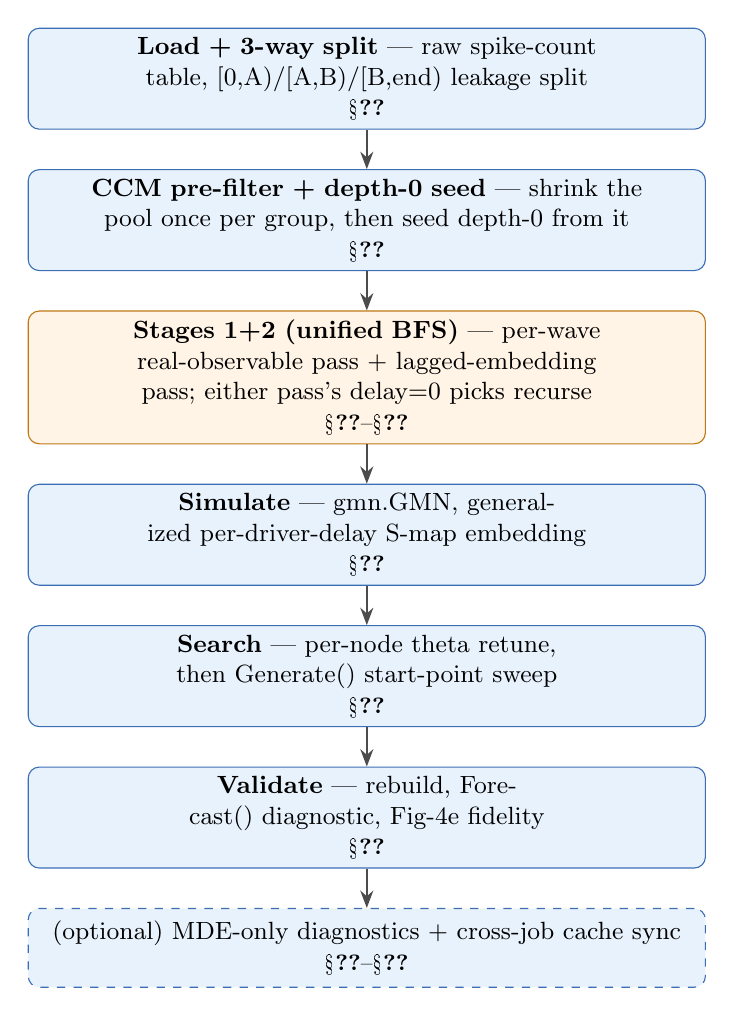
\begin{tikzpicture}[node distance=5mm]
  \node[stagebox] (s0) {\textbf{Load + 3-way split} --- raw spike-count table, [0,A){/}[A,B){/}[B,end) leakage split\\ \footnotesize \S\ref{sec:split}};
  \node[stagebox, below=of s0] (spre) {\textbf{CCM pre-filter + depth-0 seed} --- shrink the pool once per group, then seed depth-0 from it\\ \footnotesize \S\ref{sec:ccm-prefilter-section}};
  \node[stage2box, below=of spre] (s1) {\textbf{Stages 1+2 (unified BFS)} --- per-wave real-observable pass + lagged-embedding pass; either pass's delay=0 picks recurse\\ \footnotesize \S\ref{sec:stage1}--\S\ref{sec:stage2}};
  \node[stagebox, below=of s1] (s3) {\textbf{Simulate} --- gmn.GMN, generalized per-driver-delay S-map embedding\\ \footnotesize \S\ref{sec:smap}};
  \node[stagebox, below=of s3] (s4) {\textbf{Search} --- per-node theta retune, then Generate() start-point sweep\\ \footnotesize \S\ref{sec:search}};
  \node[stagebox, below=of s4] (s5) {\textbf{Validate} --- rebuild, Forecast() diagnostic, Fig-4e fidelity\\ \footnotesize \S\ref{sec:validation}};
  \node[stagebox, below=of s5, dashed] (s6) {(optional) MDE-only diagnostics + cross-job cache sync\\ \footnotesize \S\ref{sec:diagnostics}--\S\ref{sec:storage}};
  \foreach \a/\b in {s0/spre,spre/s1,s1/s3,s3/s4,s4/s5,s5/s6}
    \draw[arrow] (\a) -- (\b);
\end{tikzpicture}
\caption{The pipeline's stages, in \texttt{main()}'s actual call order. The orange box (unified Stages 1+2) is this pipeline's own novel contribution -- no notebook precedent, see Section~\ref{sec:stage1}.}
\label{fig:overview}
\end{figure}

\subsection{Relationship to the sibling pipeline}
\label{sec:sibling}
\texttt{simple-mde-gmn.py} and \texttt{tsls-mde-gmn.py} (documented separately, \texttt{docs/tsls-mde-gmn-pipeline.pdf}) both answer the causal-network question above, but differ in two load-bearing ways worth stating up front rather than discovering by surprise mid-document:
\begin{itemize}
  \item \textbf{Data representation.} The sibling pipeline TSLS-converts every candidate neuron (Time Since Last Spike -- a continuous re-encoding of a spike train, since Takens embedding needs local geometry a sparse spike train doesn't have). \textbf{This pipeline does not.} It hands \texttt{dimx.MDE} the raw, per-region-binned spike \emph{counts} directly -- confirmed by inspecting the actual input file, \texttt{J1620210605\_epoch\_8\_freq\_1\_Hz.csv}: 1-second bins, integer-valued, mean $\approx 0.12$ spikes/bin, most cells exactly 0. See the pitfall box in Section~\ref{sec:limitations} for why this asymmetry with the sibling's own stated rationale is worth a reader's attention.
  \item \textbf{MDE engine.} The sibling pipeline replaced \texttt{dimx.MDE} with a from-scratch \texttt{proper_mde} specifically so its scoring metric could be event-timing-aware (\texttt{'f1'}/\texttt{'gamma'}) rather than Pearson-only. \textbf{This pipeline still uses the original \texttt{dimx.MDE}} (Pearson correlation scoring throughout, Section~\ref{sec:dimx}) -- but compensates by replacing the sibling's other axis of rigidity: instead of one uniform, network-wide $(E,\tau)$, this pipeline builds a genuinely \emph{non-uniform, per-driver, per-delay} embedding directly from a causally-discovered graph (Sections~\ref{sec:stage1}--\ref{sec:smap}), which the sibling pipeline (inheriting \texttt{apps.CreateNetwork}'s architecture) does not do.
\end{itemize}
The two pipelines are deliberate, near-verbatim-duplicated siblings for the reasons Section~\ref{sec:sibling} of that other document gives (neither can silently break the other); a fix made in one's shared machinery -- the \texttt{pyEDM.CCM()} pool-spawn fix in particular, Section~\ref{sec:history-pool} -- must be manually ported to the other. This now includes the CCM pre-filter and its depth-0-seeding order (Section~\ref{sec:ccm-prefilter-section}) and the unified per-wave nested-MDE BFS (Sections~\ref{sec:stage1}--\ref{sec:stage2}): both pipelines share these identically, and both received the CCM-pre-filter-ordering and Stage-2-recursion fixes (Section~\ref{sec:history-prefilter-order}) together, per explicit request, precisely to keep this parity intact.

\subsection{How to read this document}
\begin{itemize}
  \item Each algorithm section opens with a plain-English statement of the problem being solved, then a numbered \textbf{Step 1 / Step 1.1 / Step 2 \ldots} breakdown of exactly what the code does, in order, using the exact function names in \texttt{scripts/src/simple-mde-gmn.py}.
  \item \tikz\node[draw=linknote, fill=linknote!6, rounded corners, inner sep=2pt]{\scriptsize\textbf{purple boxes}}; explain \emph{why} the next algorithm follows the one just described.
  \item \tikz\node[draw=badline, fill=badfill, rounded corners, inner sep=2pt]{\scriptsize\textbf{red boxes}}; flag a known risk, limitation, or open question.
  \item \tikz\node[draw=okline, fill=okfill, rounded corners, inner sep=2pt]{\scriptsize\textbf{green boxes}}; record a design decision made deliberately, with the reasoning, so it reads as a choice rather than an accident.
  \item Section~\ref{sec:outputs} is real output from an actual completed run of \emph{this exact codebase} (job 37946959) -- not a mockup, not the sibling pipeline's output, and not a hypothetical. Section~\ref{sec:history} is the single most important section for a reviewer: a chronological, no-spin account of every bug this pipeline hit, what was actually wrong (sometimes different from the first guess), and what tradeoff each fix accepted.
\end{itemize}

\newpage
% =====================================================================
\section{Data Loading and the Three-Way Temporal Split}
\label{sec:split}
% =====================================================================

\subsection{The leakage problem this split solves}
Every stage after this one either (a) discovers which neurons causally drive the targets (Stages 1--2), or (b) reports how well a network simulates the targets' future (Sections~\ref{sec:search}--\ref{sec:validation}). If the same rows of data are used for both, the reported fidelity is not a genuine out-of-sample test -- a network could look good simply because its own construction already "knew" the answer for those rows. \texttt{load_config()} and \texttt{main()} resolve one dataset-wide split, up front, and every downstream stage is threaded through it rather than improvising its own train/test boundary.

\begin{figure}[h]
\centering
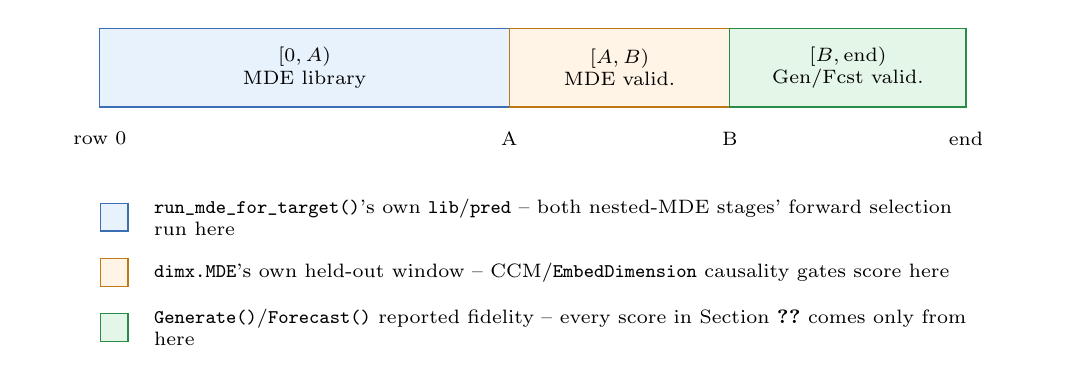
\begin{tikzpicture}[scale=1.0, every node/.style={font=\scriptsize}]
  \draw[fill=stagefill, draw=stageline] (0,0) rectangle (5.2,1);
  \node[align=center, text width=4.8cm] at (2.6,0.5) {$[0,A)$\\MDE library};
  \draw[fill=stage2fill, draw=stage2line] (5.2,0) rectangle (8.0,1);
  \node[align=center, text width=2.6cm] at (6.6,0.5) {$[A,B)$\\MDE valid.};
  \draw[fill=okfill, draw=okline] (8.0,0) rectangle (11.0,1);
  \node[align=center, text width=2.8cm] at (9.5,0.5) {$[B,\mathrm{end})$\\Gen/Fcst valid.};
  \node[below, text width=1.6cm, align=center] at (0,-0.2) {row 0};
  \node[below, text width=2.4cm, align=center] at (5.2,-0.2) {A};
  \node[below, text width=1.6cm, align=center] at (8.0,-0.2) {B};
  \node[below, text width=1.6cm, align=center] at (11.0,-0.2) {end};

  \node[rectangle, draw=stageline, fill=stagefill, minimum width=0.35cm, minimum height=0.35cm, anchor=west] (leg1) at (0,-1.4) {};
  \node[align=left, text width=10.6cm, anchor=west] at ($(leg1.east)+(0.2,0)$) {\texttt{run\_mde\_for\_target()}'s own \texttt{lib}/\texttt{pred} -- both nested-MDE stages' forward selection run here};
  \node[rectangle, draw=stage2line, fill=stage2fill, minimum width=0.35cm, minimum height=0.35cm, anchor=west] (leg2) at (0,-2.1) {};
  \node[align=left, text width=10.6cm, anchor=west] at ($(leg2.east)+(0.2,0)$) {\texttt{dimx.MDE}'s own held-out window -- CCM/\texttt{EmbedDimension} causality gates score here};
  \node[rectangle, draw=okline, fill=okfill, minimum width=0.35cm, minimum height=0.35cm, anchor=west] (leg3) at (0,-2.8) {};
  \node[align=left, text width=10.6cm, anchor=west] at ($(leg3.east)+(0.2,0)$) {\texttt{Generate()}/\texttt{Forecast()} reported fidelity -- every score in Section~\ref{sec:validation} comes only from here};
\end{tikzpicture}
\caption{The three-way split: \texttt{PREDICTION\_START}=A $= \texttt{LIB\_RATIO} \times \mathrm{len(df)}$, \texttt{PREDICTION\_LENGTH}=B$-$A, \texttt{GENERATE\_VALIDATION\_START}=B. Network construction (Stages 1--2) never sees past B; every Generate()/Forecast() score is computed only on $[B, \mathrm{end})$.}
\label{fig:split}
\end{figure}

\subsection{Algorithm: the split's own arithmetic (\texttt{main()})}
\begin{steps}
\item \texttt{PREDICTION\_START} (A) $= \mathrm{round}(\texttt{LIB\_RATIO} \times \texttt{len(df)})$.
\item \texttt{PREDICTION\_LENGTH} (B$-$A) $= \mathrm{round}((\texttt{len(df)} - A) \times \texttt{MDE\_VALIDATION\_RATIO})$.
\item \texttt{GENERATE\_VALIDATION\_START} (B) $= A + (B{-}A)$; \texttt{GENERATE\_VALIDATION\_LENGTH} $= \texttt{len(df)} - B$.
\item \texttt{GENERATE\_LENGTH} (how many steps one \texttt{Generate()} call free-runs): 0 means "use the whole [B,end) segment"; anything larger than \texttt{GENERATE\_VALIDATION\_LENGTH} is clamped down to it, since there would be no real data left to score the extra steps against.
\end{steps}

\pitfallbox{This clamp is not hypothetical -- it applies to the job in flight right now:}{The current data file (\texttt{J1620210605\_epoch\_8\_freq\_1\_Hz.csv}) has 1{,}199 rows. At the sbatch script's own \texttt{LIB\_RATIO=0.75}/\texttt{MDE\_VALIDATION\_RATIO=0.5}, A=899, B=1049, and \texttt{GENERATE\_VALIDATION\_LENGTH} is only 150 rows -- so the configured \texttt{GENERATE\_LENGTH=300} silently clamps down to 150 the moment \texttt{main()} runs. Every Generate()/Forecast() diagnostic for this run is therefore over a 150-step window, not the 300 the sbatch parameter block implies; a reader checking that file alone would get the wrong number.}

\subsection{Algorithm: \texttt{run\_mde\_for\_target}'s own leakage guard}
\label{sec:leakage-guard}
The three-way split above only sets the boundaries; this is the function that actually enforces them, and it is worth reading carefully because the obvious-looking mechanism (passing \texttt{lib}/\texttt{pred} range strings to \texttt{dimx.MDE}) is \emph{not} what does the real work.
\begin{steps}
\item Slice \texttt{mde\_df = df[[target] + observable\_columns].iloc[:A + (B{-}A)]} -- i.e. physically truncate the DataFrame object at row B before it is ever handed to \texttt{dimx.MDE}.
\item Pass \texttt{lib=[warmup+1, A]} and \texttt{pred=[A+1, B-Tp]} (the \texttt{-Tp} so the last validated row's own $t{+}\texttt{Tp}$ label can never land at or past B either).
\end{steps}
\pitfallbox{The physical truncation in Step 1 is the actual guard, not the lib/pred strings in Step 2:}{Confirmed by reading \texttt{pyEDM/CCM.py} directly: \texttt{dimx.MDE}'s own internal \texttt{CCM()} causality-validation call ignores the \texttt{lib}/\texttt{pred} bounds it's given and samples its library/prediction sets from \emph{whatever DataFrame object it's handed} -- so if \texttt{mde\_df} still contained rows past B, \texttt{CCM()} could sample from segment 3 regardless of what \texttt{lib}/\texttt{pred} say. \texttt{exclusionRadius} doesn't help either: it only ever narrows an already-available candidate set, never expands it past what the DataFrame itself contains. This is why Step 1's slice exists as a completely separate line from Step 2's arguments, not merged into one call.}

\linknote{Every row from 0 to B is now available for MDE to search (Stages 1--2 next), and every row from B onward is guaranteed untouched until the Generate()/Forecast() validation stages (Section~\ref{sec:validation}) -- which is exactly the property a genuine out-of-sample causal-network test needs.}

\newpage
% =====================================================================
\section{Before Stage 1: the CCM Pre-Filter and the Depth-0 MDE Seed}
\label{sec:ccm-prefilter-section}
% =====================================================================
Two things happen in \texttt{main()} after the leakage-safe split (Section~\ref{sec:split}) but before Stage 1's BFS (Section~\ref{sec:stage1}) ever runs: the candidate pool is shrunk by a cheap CCM screen, and each target's own depth-0 driver search is seeded from that same shrunk pool. Both are explicit, main()-level steps for the same underlying reason: neither is something the BFS's own generic, per-node machinery can do on its own.

\subsection{The CCM pre-filter: shrinking the candidate pool before any MDE runs}
\label{sec:ccm-prefilter}
\texttt{REGION\_CHANNEL\_CAP} can offer hundreds of channels as MDE candidates -- \texttt{dimx.MDE}'s own forward-selection ranking cost grows with candidate-pool size at every dimension, so a large pool is expensive well before any driver is actually selected. \texttt{ccm\_prefilter\_observables()} runs a single, cheap CCM(observable $\to$ target) skill check per candidate, once per \texttt{target\_groups\_for\_mode()} group, and keeps only the candidates that cross-map at least one target in the group above \texttt{CCM\_PREFILTER\_RHO\_MIN} -- a coarse relevance screen, not a substitute for \texttt{dimx.MDE}'s own causality-gated selection (Section~\ref{sec:dimx}).

\begin{steps}
\item For every group from \texttt{target\_groups\_for\_mode()}, slice the leakage-safe MDE library+validation window \texttt{df.iloc[:A+(B{-}A)]} (Section~\ref{sec:leakage-guard}) and convert \texttt{LIBSIZE\_RATIOS} (fractions of \texttt{PREDICTION\_START}, i.e.\ of segment $[0,A)$) into actual library sizes, deduped and floored at 10 rows.
\item For every candidate, run one \texttt{pyEDM.CCM} per target at a static \texttt{CCM\_PREFILTER\_E} (no per-candidate auto-select -- would defeat the point of a \emph{cheap} filter), \texttt{tau=-1}/\texttt{sample=20} matching \texttt{dimx.MDE}'s own unoverridden pyEDM defaults, and average the score across the swept library sizes.
\item Average each candidate's per-target scores across the group; keep the candidate if that average is $\geq$ \texttt{CCM\_PREFILTER\_RHO\_MIN}. \texttt{CCM\_PREFILTER\_RHO\_MIN=0} disables the filter entirely (the pool passes through unchanged).
\item Parallelized over \emph{candidates} via a \texttt{ProcessPoolExecutor} (fork context, \texttt{\_mde\_wave\_worker\_init} initializer -- the same sequential-\texttt{CCM()} patch every other wave pool in this file already applies, Section~\ref{sec:history-pool}); each worker computes one candidate's score against every target sequentially.
\end{steps}

\begin{figure}[H]
\centering
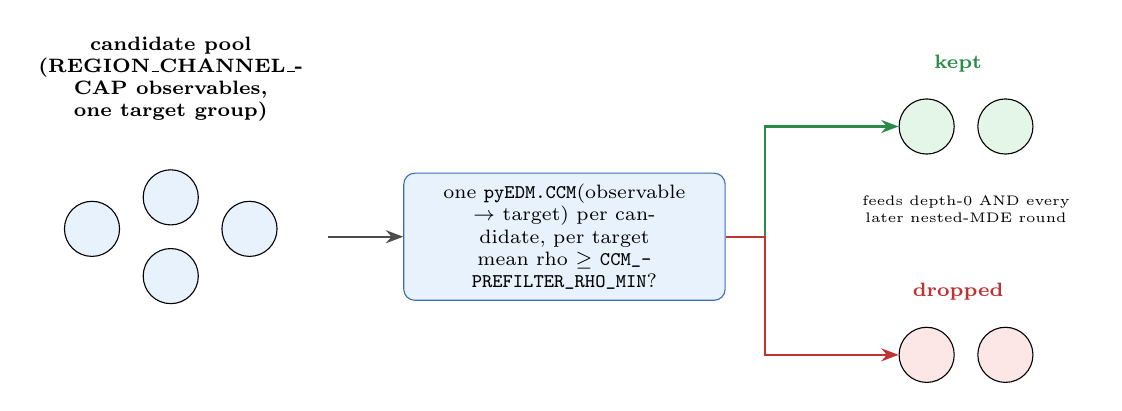
\begin{tikzpicture}[every node/.style={font=\scriptsize}]
  \node[font=\bfseries\scriptsize, align=center, text width=3.4cm] at (-4.6,3.3) {candidate pool\\(REGION\_CHANNEL\_CAP observables, one target group)};
  \node[circle, draw, fill=stagefill, minimum size=7mm] (o1) at (-5.6,1.4) {};
  \node[circle, draw, fill=stagefill, minimum size=7mm] (o2) at (-4.6,1.8) {};
  \node[circle, draw, fill=stagefill, minimum size=7mm] (o3) at (-3.6,1.4) {};
  \node[circle, draw, fill=stagefill, minimum size=7mm] (o4) at (-4.6,0.8) {};
  \node[smallbox, text width=3.8cm] (filt) at (0.4,1.3) {one \texttt{pyEDM.CCM}(observable $\to$ target) per candidate, per target\\mean rho $\geq$ \texttt{CCM\_PREFILTER\_RHO\_MIN}?};
  \draw[arrow] (-2.6,1.3) -- (filt);
  \node[font=\bfseries\scriptsize, okline] at (5.4,3.5) {kept};
  \node[circle, draw, fill=okfill, minimum size=7mm] (k1) at (5.0,2.7) {};
  \node[circle, draw, fill=okfill, minimum size=7mm] (k2) at (6.0,2.7) {};
  \node[font=\tiny, align=center, text width=3.0cm] at (5.5,1.65) {feeds depth-0 AND every later nested-MDE round};
  \draw[arrow, okline] (filt.east) -- ++(0.5,0) |- (k1);
  \node[font=\bfseries\scriptsize, badline] at (5.4,0.6) {dropped};
  \node[circle, draw, fill=badfill, minimum size=7mm] (d1) at (5.0,-0.2) {};
  \node[circle, draw, fill=badfill, minimum size=7mm] (d2) at (6.0,-0.2) {};
  \draw[arrow, badline] (filt.east) -- ++(0.5,0) |- (d1);
\end{tikzpicture}
\caption{\texttt{ccm\_prefilter\_observables()}: a coarse, cheap CCM relevance screen run once per target group, before depth-0 or any nested-MDE round ever searches the pool.}
\label{fig:ccm-prefilter}
\end{figure}

\subsection{Why depth-0 has to be computed explicitly, right here}
\label{sec:why-depth0-explicit}
\texttt{build\_nested\_mde\_network()}'s BFS (Section~\ref{sec:stage1}) is a generic, per-\emph{node} algorithm: every node it processes, target or driver alike, goes through the identical per-wave machinery, with one deliberate shortcut -- reuse a precomputed result instead of calling \texttt{dimx.MDE} again when \texttt{depth==0 and node in mde\_results}. That shortcut is what makes depth-0 special, and it is also exactly why depth-0 cannot simply be left for the BFS to discover on its own the first time it reaches a target node, rather than diving straight from the CCM pre-filter into network construction.

\begin{steps}
\item The CCM pre-filter (Section~\ref{sec:ccm-prefilter}) is a \emph{group}-level operation -- it has to run once per \texttt{target\_groups\_for\_mode()} group, against every target in that group at once, before any individual node's MDE call happens. The BFS itself has no group-level entry point: it only ever sees one node at a time, so it has nowhere to run a once-per-group filter from.
\item Whatever pool that pre-filter produces has to be the \emph{same} pool every later round searches -- depth-0's own selection and every deeper nested-MDE round must all be choosing from identical candidates, or a column one round accepted can go missing from another round's own view of the universe.
\item \texttt{main()} therefore resolves \texttt{filtered\_pools[group]} once, up front, and passes that \emph{same} object both to the depth-0 seed call (\texttt{run\_mde\_for\_target()}) and to \texttt{build\_network()}'s own \texttt{observable\_columns} argument, which \texttt{build\_nested\_mde\_network()} then uses for every subsequent wave.
\end{steps}

\begin{figure}[H]
\centering
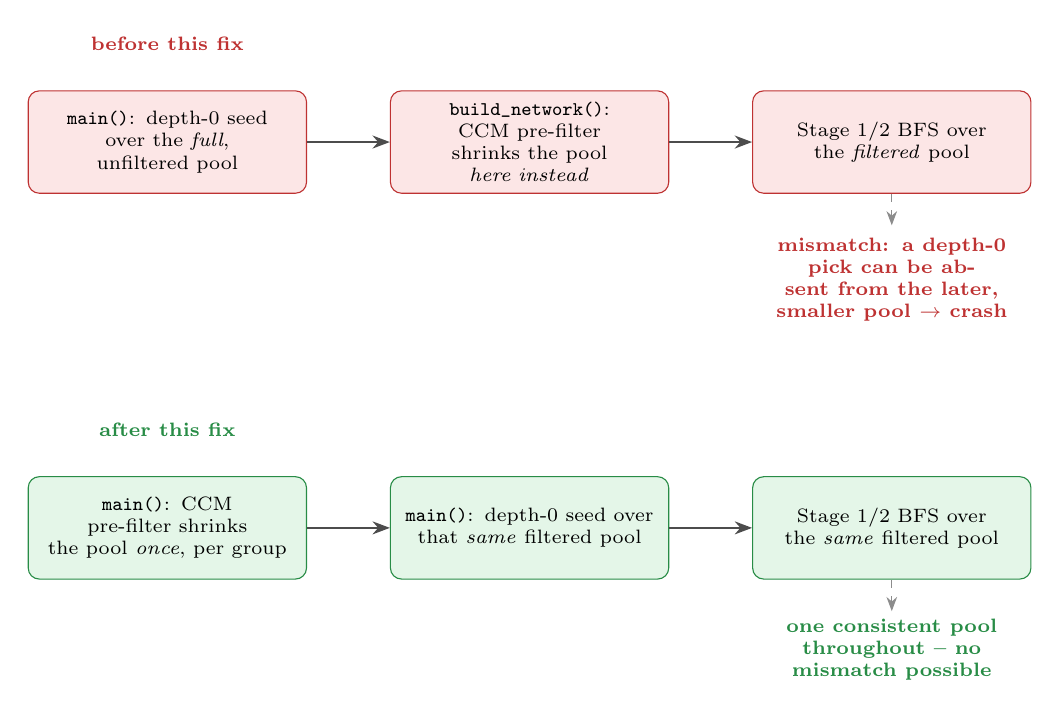
\begin{tikzpicture}[every node/.style={font=\scriptsize}]
  \node[font=\bfseries\scriptsize, badline] at (-5.6,3.75) {before this fix};
  \node[rectangle, draw=badline, fill=badfill, rounded corners, text width=3.3cm, minimum height=1.3cm, align=center] (old1) at (-5.6,2.5) {\texttt{main()}: depth-0 seed\\over the \emph{full}, unfiltered pool};
  \node[rectangle, draw=badline, fill=badfill, rounded corners, text width=3.3cm, minimum height=1.3cm, align=center] (old2) at (-1.0,2.5) {\texttt{build\_network()}: CCM pre-filter\\shrinks the pool \emph{here instead}};
  \node[rectangle, draw=badline, fill=badfill, rounded corners, text width=3.3cm, minimum height=1.3cm, align=center] (old3) at (3.6,2.5) {Stage 1/2 BFS over\\the \emph{filtered} pool};
  \draw[arrow] (old1) -- (old2);
  \draw[arrow] (old2) -- (old3);
  \draw[faintarrow] (old3.south) -- ++(0,-0.4);
  \node[font=\scriptsize\bfseries, badline, align=center, text width=3.4cm] at (3.6,0.75) {mismatch: a depth-0 pick can be absent from the later, smaller pool $\to$ crash};

  \node[font=\bfseries\scriptsize, okline] at (-5.6,-1.15) {after this fix};
  \node[rectangle, draw=okline, fill=okfill, rounded corners, text width=3.3cm, minimum height=1.3cm, align=center] (new1) at (-5.6,-2.4) {\texttt{main()}: CCM pre-filter shrinks\\the pool \emph{once}, per group};
  \node[rectangle, draw=okline, fill=okfill, rounded corners, text width=3.3cm, minimum height=1.3cm, align=center] (new2) at (-1.0,-2.4) {\texttt{main()}: depth-0 seed over\\that \emph{same} filtered pool};
  \node[rectangle, draw=okline, fill=okfill, rounded corners, text width=3.3cm, minimum height=1.3cm, align=center] (new3) at (3.6,-2.4) {Stage 1/2 BFS over\\the \emph{same} filtered pool};
  \draw[arrow] (new1) -- (new2);
  \draw[arrow] (new2) -- (new3);
  \draw[faintarrow] (new3.south) -- ++(0,-0.4);
  \node[font=\scriptsize\bfseries, okline, align=center, text width=3.4cm] at (3.6,-3.95) {one consistent pool throughout -- no mismatch possible};
\end{tikzpicture}
\caption{Reordering the CCM pre-filter fixed a real crash (\texttt{CA1\_22}, Section~\ref{sec:history-prefilter-order}): depth-0's own candidate pool now comes from the exact same filtering pass every later nested-MDE round uses, instead of being computed separately, earlier, against a different (unfiltered) pool.}
\label{fig:prefilter-ordering}
\end{figure}

\pitfallbox{This is not a hypothetical failure mode -- it crashed real jobs:}{See Section~\ref{sec:history-prefilter-order} for the full symptom/investigation/decision writeup: \texttt{observable\_and\_delay()} raised \texttt{ValueError: invalid literal for int() with base 10: 'CA1\_22'} when a depth-0-selected real observable, chosen against the old code's unfiltered pool, turned out absent from Stage 1/2's own (filtered) \texttt{raw\_columns} list.}

\newpage
% =====================================================================
\section{Stage 1: Nested-MDE Backbone Discovery}
\label{sec:stage1}
% =====================================================================

\subsection{Why this has no notebook precedent}
The reference notebook (and the sibling pipeline) build a network by running CCM over the \emph{union} of each target's MDE-selected columns, then handing an $N \times N$ interaction matrix to \texttt{apps.CreateNetwork} for greedy, acyclic graph assembly (documented in the sibling's own Section 5). \texttt{build_nested_mde_network()} replaces that whole approach: it discovers the network's topology directly from repeated \texttt{dimx.MDE} calls -- no CCM, no interaction matrix, no \texttt{apps.CreateNetwork} anywhere in \texttt{MODE='MDE-GMN'}. Each target's MDE-selected drivers themselves become new MDE targets, recursively, for \texttt{NESTED\_M} further rounds -- an algorithm this project built from scratch, per explicit direction, specifically because MDE's own forward selection is already a legitimate way to discover a driver, and re-deriving the same structure from an interaction matrix afterward would be redundant work over the same underlying question.

\subsection{Algorithm: \texttt{build\_nested\_mde\_network} -- the unified per-wave BFS}
As of 2026-08-25, Stage 1 and Stage 2 are unified into \textbf{one} BFS: every wave, every node gets \emph{both} a Stage-1-style pass and a Stage-2-style pass, not one pass in a separate, later sweep (Section~\ref{sec:stage2} covers exactly what this changed and why).
\begin{steps}
\item \textbf{Depth 0:} \texttt{main()} already computed \texttt{mde\_results} for every target before this BFS ever runs -- one \texttt{dimx.MDE} call per target, selecting up to \texttt{MDE\_D} distinct real observables from the CCM-pre-filtered candidate pool (Section~\ref{sec:ccm-prefilter}, excluding the target itself). The BFS simply reuses that precomputed result as its depth-0 Stage-1 pass, rather than paying for it twice -- but it still runs a Stage-2 pass at depth 0, same as every other depth (Section~\ref{sec:stage2}).
\item \textbf{Every wave, every node:} a \textbf{Stage 1 pass} (real-observable-only candidates, so every accepted edge necessarily has delay 0) \emph{and} a \textbf{Stage 2 pass} (lagged -- or lagged+real when \texttt{STAGE2\_ALLOW\_REAL\_OBSERVABLES=true} -- candidates drawn from the whole CCM-pre-filtered observable universe). Both go through the same \texttt{run\_mde\_for\_target()}; the Stage 2 pool for a wave is submitted only after that wave's Stage 1 pool has fully returned, so edge acceptance (next step) always sees both results together.
\item \textbf{Depth 1..NESTED\_M:} every driver selected \emph{at delay 0}, by \emph{either} pass, in the previous depth becomes a new MDE target in its own right, again getting both passes. \texttt{NESTED\_M=0} is a sentinel for "uncapped" -- nesting continues until it runs out on its own rather than stopping at a fixed round count.
\item \textbf{Edge acceptance} (\texttt{\_accept\_mde\_result\_edges()}, shared by both passes): for every column MDE selected, reject it as a self-loop (belt-and-suspenders); reject it if its \emph{marginal} MDE rho gain ($\mathrm{gain}_d = \mathrm{MDErho}[d]-\mathrm{MDErho}[d{-}1]$) is \texttt{NaN}; otherwise tentatively add the edge to a shared \texttt{networkx.MultiDiGraph} and immediately check \texttt{nx.is\_directed\_acyclic\_graph()} -- if the edge would close a cycle, remove it by its specific key and move on. Applied to the Stage 1 pass's result first, then the Stage 2 pass's, so acyclicity is checked across both passes' edges together.
\item \textbf{Continue nesting} only through edges accepted at \textbf{delay 0}, from either pass: a driver selected at a nonzero delay is added to the graph as a terminal edge, never itself re-MDE'd (see the decision box below).
\end{steps}

\begin{figure}[h]
\centering
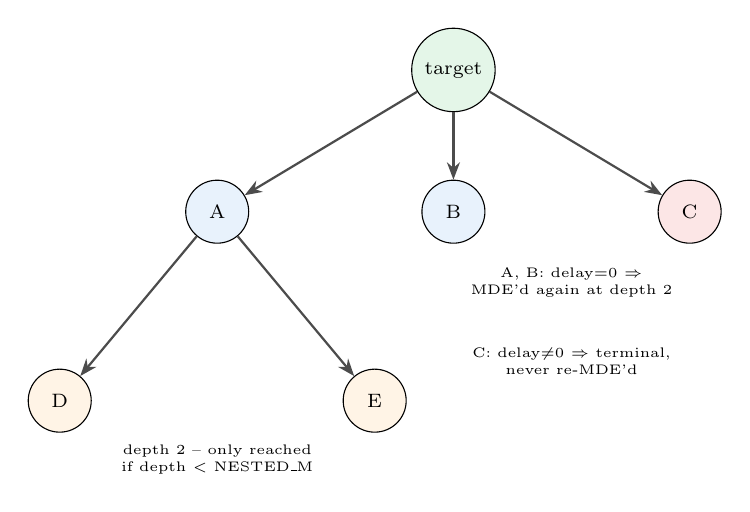
\begin{tikzpicture}[every node/.style={font=\scriptsize}]
  % depth 0
  \node[circle, draw, fill=okfill, minimum size=8mm] (root) at (4.2,4.4) {target};
  % depth 1
  \node[circle, draw, fill=stagefill, minimum size=8mm] (a) at (1.2,2.6) {A};
  \node[circle, draw, fill=stagefill, minimum size=8mm] (b) at (4.2,2.6) {B};
  \node[circle, draw, fill=badfill, minimum size=8mm] (c) at (7.2,2.6) {C};
  \draw[arrow] (root) -- (a);
  \draw[arrow] (root) -- (b);
  \draw[arrow] (root) -- (c);
  \node[font=\tiny, align=center, text width=2.6cm] at (5.7,1.7) {A, B: delay=0 $\Rightarrow$ MDE'd again at depth 2};
  \node[font=\tiny, align=center, text width=2.6cm] at (5.7,0.7) {C: delay$\ne$0 $\Rightarrow$ terminal, never re-MDE'd};
  % depth 2, children of A only
  \node[circle, draw, fill=stage2fill, minimum size=8mm] (d) at (-0.8,0.2) {D};
  \node[circle, draw, fill=stage2fill, minimum size=8mm] (e) at (3.2,0.2) {E};
  \draw[arrow] (a) -- (d);
  \draw[arrow] (a) -- (e);
  \node[font=\tiny, align=center, text width=3.8cm] at (1.2,-0.55) {depth 2 -- only reached if depth $<$ NESTED\_M};
\end{tikzpicture}
\caption{The BFS's depth/delay rule: only delay-0 accepted edges (A, B) enqueue their driver for further nesting; a nonzero-delay edge (C) terminates that branch immediately. This rule applies identically regardless of \emph{which} pass -- Stage 1 or Stage 2 -- produced the edge (Section~\ref{sec:stage2}).}
\label{fig:stage1-bfs}
\end{figure}

\decisionbox{Why only delay=0 continues the search:}{A driver selected at a nonzero delay stands in for an unobserved dimension of the true state space -- a placeholder, per generalized embedding theory (Deyle \& Sugihara 2011), not a physical variable whose own causal history is worth discovering. Nesting into it would search for "the causal history of a lag," which isn't a meaningful question. Nodes reached only via a delay$\ne$0 edge still simulate fine (Section~\ref{sec:smap}): they get an unconditional self-embedding the same way any driverless leaf node already does.}

\decisionbox{Why a \texttt{MultiDiGraph}, not a \texttt{DiGraph}:}{Per explicit direction, the same observable can drive one node at several different delays at once -- each is kept as its own separate edge (visualized as separate colored arcs in Figure~\ref{fig:real-network}), not deduplicated to one edge with one delay.}

\subsection{Algorithm: parallelization within one wave}
Every node at the same BFS depth is MDE-independent of every other \emph{node}, so each pass (Stage 1, then Stage 2) is submitted concurrently via its own \texttt{ProcessPoolExecutor} -- the Stage 2 pass intentionally waits for the whole wave's Stage 1 pass to return first, so both passes' results are available together when edge acceptance runs. Within a pass, outer (per-node) and inner (each node's own \texttt{CrossMapColumns}) parallelism are split \emph{adaptively per wave} rather than both left at the full core count -- \texttt{outer\_workers = min(len(wave), cores)}, \texttt{inner\_cores = max(1, cores // outer\_workers)} -- specifically to avoid reproducing the outer$\times$inner pool-squaring blowup this project hit once already (Section~\ref{sec:history-pool}).

\begin{figure}[H]
\centering
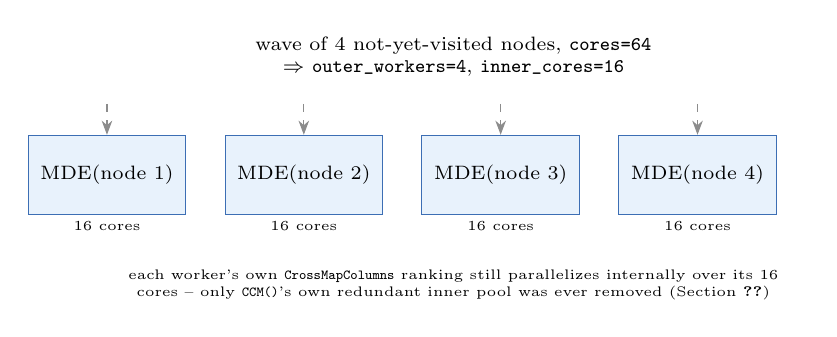
\begin{tikzpicture}[every node/.style={font=\scriptsize}]
  \node[align=center] at (4.4,3.5) {wave of 4 not-yet-visited nodes, \texttt{cores=64}\\$\Rightarrow$ \texttt{outer\_workers=4}, \texttt{inner\_cores=16}};
  \foreach \i/\x in {1/0,2/2.5,3/5,4/7.5} {
    \node[rectangle, draw=stageline, fill=stagefill, minimum width=2cm, minimum height=1cm] (w\i) at (\x,2) {MDE(node \i)};
    \node[font=\tiny, align=center] at (\x,1.35) {16 cores};
    \draw[faintarrow] (\x,2.9) -- (w\i);
  }
  \node[font=\tiny, text width=8.8cm, align=center] at (4.4,0.6) {each worker's own \texttt{CrossMapColumns} ranking still parallelizes internally over its 16 cores -- only \texttt{CCM()}'s own redundant inner pool was ever removed (Section~\ref{sec:history-pool})};
\end{tikzpicture}
\caption{One BFS wave's adaptive core split: wide waves lean on more outer workers, each single-threaded-ish inward; a narrow wave instead hands its one or two calls a much larger inner-core budget.}
\label{fig:wave-split}
\end{figure}

\pitfallbox{A single degenerate node used to be able to crash the entire job:}{See Section~\ref{sec:history-crash} -- job 37946756 lost 1 day 11 hours of compute to one node's \texttt{dimx.Run.Run()} hitting an all-NaN rho column deep inside a third-party library, an exception that propagated straight out of the wave's \texttt{ProcessPoolExecutor} and killed every already-completed node's work alongside it. Every wave-consumption loop (both passes, and \texttt{main()}'s own depth-0 seed) now catches that per-node exception and substitutes \texttt{\_failed\_mde\_result()} -- shaped identically to a legitimate zero-driver selection -- so one bad node dead-ends cleanly instead of taking the run down.}

\linknote{Every wave now produces both a real-observable backbone edge set and a lagged-embedding edge set together. What's still open is exactly what changed about how the Stage 2 pass's own real-observable picks behave -- that's the whole subject of Section~\ref{sec:stage2}.}

\newpage
% =====================================================================
\section{Stage 2: Lagged-Embedding Attachment}
\label{sec:stage2}
% =====================================================================

\subsection{The problem Stage 2 solves}
Stage 1's own picks tell you \emph{which} real observables matter and how they connect. They say nothing about \emph{how far back in time} each connection should look, or which additional variables -- not necessarily direct Stage-1 neighbors -- best explain a node's own recent history once its embedding is allowed to be genuinely non-uniform (a generalized/non-uniform Takens embedding, Deyle \& Sugihara 2011: different driving variables, and even repeats of the same driver, can each carry their own delay instead of sharing one lag network-wide). The Stage 2 pass runs one \texttt{dimx.MDE} round per node, every wave, to answer that.

\subsection{Algorithm: the Stage 2 pass}
\begin{steps}
\item For every node in the current wave (targets included, every depth including 0), build a candidate pool of \texttt{lag\_set} $\times$ \emph{every} real observable in the CCM-pre-filtered universe -- deliberately not restricted to that node's own Stage-1 neighbors, per explicit direction, so a node's best lagged predictor can come from anywhere in the observable universe.
\item Run one \texttt{dimx.MDE} round (same \texttt{run\_mde\_for\_target()}, same leakage guard as the Stage 1 pass, \texttt{cache\_stage='stage2'} so its cache files never collide with Stage 1's) selecting up to \texttt{MDE\_D} lagged columns.
\item Feed every result through the \emph{same} \texttt{\_accept\_mde\_result\_edges()} as the Stage 1 pass -- self-loop guard, NaN-gain rejection, eager cycle rejection all apply identically.
\item \texttt{STAGE2\_ALLOW\_REAL\_OBSERVABLES=false} (the default) keeps Stage 2's own candidate pool lag-only, so it can only ever produce delay$\ne$0 edges; set it \texttt{true} to let Stage 2's candidate pool also include delay=0 (real-observable) columns.
\end{steps}

\begin{figure}[h]
\centering
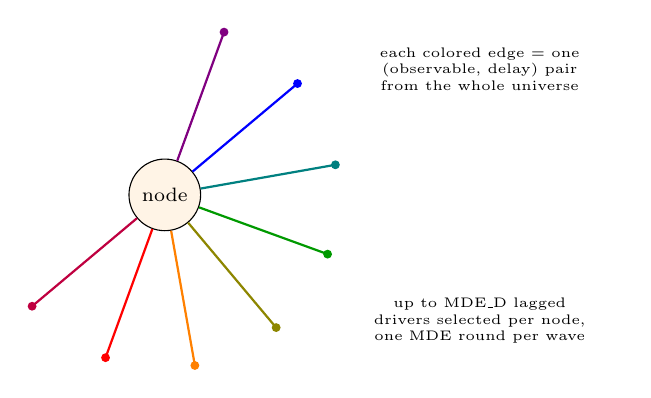
\begin{tikzpicture}[every node/.style={font=\scriptsize}]
  \node[circle, draw, fill=stage2fill, minimum size=9mm] (n) at (0,0) {node};
  \foreach \i/\a/\c in {1/70/violet,2/40/blue,3/10/teal,4/-20/green!60!black,5/-50/olive,6/-80/orange,7/-110/red,8/-140/purple}
    {
      \coordinate (p\i) at ({\a}:2.2cm);
      \draw[\c, thick] (p\i) -- (n);
      \fill[\c] (p\i) circle (1.6pt);
    }
  \node[align=center, font=\tiny, text width=3.4cm] at (4.0,1.6) {each colored edge = one\\(observable, delay) pair\\from the whole universe};
  \node[align=center, font=\tiny, text width=3.4cm] at (4.0,-1.6) {up to MDE\_D lagged\\drivers selected per node,\\one MDE round per wave};
\end{tikzpicture}
\caption{The Stage 2 pass, schematically: one node acquires several lagged coordinates, each independently chosen from every real observable at every candidate delay -- not limited to that node's own Stage-1 neighborhood. Figure~\ref{fig:real-network} shows what this actually looks like on real data.}
\label{fig:stage2-schematic}
\end{figure}

\decisionbox{Why search the whole universe, not just each node's own neighbors:}{A node's best lagged predictor is an empirical question, not something to presuppose from Stage 1's own (real-observable-only, delay-0) topology. Per explicit direction, restricting Stage 2 to each node's already-known neighbors would bias the embedding toward whatever Stage 1 happened to find first, rather than letting MDE search freely over delay as its own dimension.}

\subsection{What changed: Stage 2's own real-observable picks now recurse}
\label{sec:stage2-recursion}
Before 2026-08-25, Stage 1 ran its \emph{entire} BFS to completion first, and only then did a separate function, \texttt{attach\_lag\_embeddings()}, run the Stage 2 pass exactly once, over Stage 1's final node set. A Stage-2-selected real observable (only possible with \texttt{STAGE2\_ALLOW\_REAL\_OBSERVABLES=true}) was accepted as a real edge into the graph, but was \emph{always} a dead-end leaf -- it was never itself re-searched for its own further drivers, unlike an identical-looking real observable Stage 1 happened to select. Review found this did not match the intended algorithm: a delay=0 driver is a delay=0 driver regardless of which pass found it, and both ought to be treated identically. The two passes are now unified into one BFS (Section~\ref{sec:stage1}) specifically so that a Stage-2 real-observable pick enqueues its own next-depth MDE round exactly like a Stage-1 pick always did.

\begin{figure}[H]
\centering
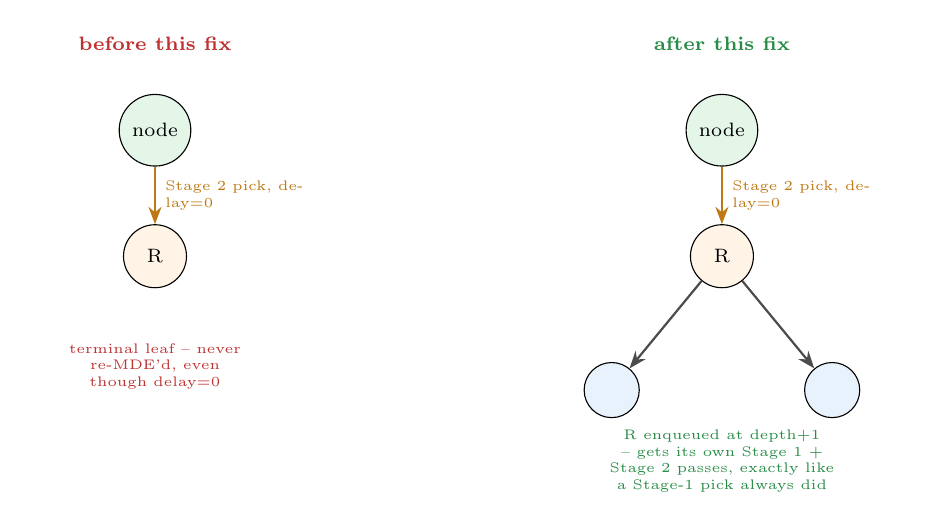
\begin{tikzpicture}[every node/.style={font=\scriptsize}]
  \node[font=\bfseries\scriptsize, badline] at (-3.6,3.1) {before this fix};
  \node[circle, draw, fill=okfill, minimum size=8mm] (n1) at (-3.6,2.0) {node};
  \node[circle, draw, fill=stage2fill, minimum size=8mm] (r1) at (-3.6,0.4) {R};
  \draw[arrow, stage2line] (n1) -- (r1) node[midway, right, font=\tiny, text width=2.2cm] {Stage 2 pick, delay=0};
  \node[font=\tiny, badline, align=center, text width=3.0cm] at (-3.6,-1.0) {terminal leaf -- never re-MDE'd, even though delay=0};

  \node[font=\bfseries\scriptsize, okline] at (3.6,3.1) {after this fix};
  \node[circle, draw, fill=okfill, minimum size=8mm] (n2) at (3.6,2.0) {node};
  \node[circle, draw, fill=stage2fill, minimum size=8mm] (r2) at (3.6,0.4) {R};
  \draw[arrow, stage2line] (n2) -- (r2) node[midway, right, font=\tiny, text width=2.2cm] {Stage 2 pick, delay=0};
  \node[circle, draw, fill=stagefill, minimum size=7mm] (x1) at (2.2,-1.3) {};
  \node[circle, draw, fill=stagefill, minimum size=7mm] (x2) at (5.0,-1.3) {};
  \draw[arrow] (r2) -- (x1);
  \draw[arrow] (r2) -- (x2);
  \node[font=\tiny, okline, align=center, text width=3.4cm] at (3.6,-2.2) {R enqueued at depth+1 -- gets its own Stage 1 + Stage 2 passes, exactly like a Stage-1 pick always did};
\end{tikzpicture}
\caption{The fix, schematically: a delay=0 real-observable pick from the Stage 2 pass (R) used to be a permanent dead end; it now recurses into its own further nested-MDE round, same as any Stage-1 pick.}
\label{fig:stage2-recursion-fix}
\end{figure}

\decisionbox{Both passes share one depth budget and one set of BFS termination conditions:}{\texttt{NESTED\_M} caps (or, at 0, leaves uncapped) how many \emph{additional} rounds either pass's delay=0 picks may trigger -- there is no separate budget for "Stage-1-discovered depth" versus "Stage-2-discovered depth." The BFS ends when every live node's own most recent round, across both passes, either selected zero drivers, selected only \texttt{NaN}-gain drivers, or selected only nonzero-delay drivers.}

\subsection{Algorithm: \texttt{derive\_lag\_set} -- resolving the candidate delays}
\begin{steps}
\item \texttt{DELAY\_SOURCE='lag\_mode'} (default): a \emph{bound} on the deepest lag magnitude is set by \texttt{LAG\_MODE} -- \texttt{'generation\_length\_adjusted'} (default) ties it to \texttt{GENERATE\_LENGTH}, so the deepest embedding coordinate never reaches further back than one full \texttt{Generate()} run needs; \texttt{'every\_lag\_possible'} instead reaches as deep as the MDE library segment $[0,A)$ structurally allows.
\item That bound is then sampled every \texttt{LAG\_STEP} rows (\texttt{LAG\_DENSITY='strided'}, default) or every single integer lag (\texttt{'dense'}).
\item \texttt{DELAY\_SOURCE='explicit'} (legacy): use the hand-picked \texttt{DELAY\_SET} list directly instead of any of the above.
\end{steps}
\pitfallbox{\texttt{LAG\_STEP=1} is forced for this pipeline's current runs, per explicit direction:}{This makes \texttt{LAG\_MODE}'s bound dense regardless of \texttt{LAG\_DENSITY} -- every consecutive row is its own candidate delay. At full scale (\texttt{REGION\_CHANNEL\_CAP=999}, $\approx$468 real observables $\times$ up to \texttt{GENERATE\_LENGTH} lags) this is a genuinely large candidate pool per Stage-2 node -- see the resource-sizing history in Section~\ref{sec:history-resources} for the real, measured cost this produces.}

\linknote{Both passes mutate the same \texttt{MultiDiGraph} in place. By the time \texttt{build\_nested\_mde\_network()} returns, that graph -- not an interaction matrix, not a call to \texttt{apps.CreateNetwork} -- \emph{is} the network. It still needs a way to actually simulate: gmn's own \texttt{Embed(E, tau, columns)} call assumes one uniform embedding, which this graph does not have. Section~\ref{sec:smap} is the patch that lets gmn simulate a genuinely non-uniform one.}

\newpage
% =====================================================================
\section{dimx.MDE: The Selection Engine Both Stages Share}
\label{sec:dimx}
% =====================================================================
Unlike the sibling pipeline (which replaced this engine with a from-scratch \texttt{proper_mde}, Section~\ref{sec:sibling}), this pipeline still calls the original third-party \texttt{dimx.MDE} unmodified, for every MDE call in both stages.

\subsection{The two-part selection dimx.MDE performs, per dimension}
\begin{steps}
\item \textbf{Ranking:} at dimension $d$, every not-yet-selected candidate is tried prepended to the current selection, scored by \texttt{CrossMapColumns} (Pearson correlation, ranking against the target), and sorted best-first.
\item \textbf{Causality gate:} walk the ranked list best-first; for each, run \texttt{EmbedDimension} then \texttt{CCM} (the sibling document's own development-history section records a real episode of this exact gate being wrongly disabled and then correctly restored, worth reading before ever touching this gate here); accept the \emph{first} candidate that passes, not necessarily the single best-ranked one.
\end{steps}
This pipeline supplies \texttt{embedDimRhoMin}/\texttt{crossMapRhoMin} as the acceptance thresholds and \texttt{Tp} (prediction interval, default 1 -- see the pitfall box below) as the horizon every candidate is ranked/validated against.

\begin{figure}[H]
\centering
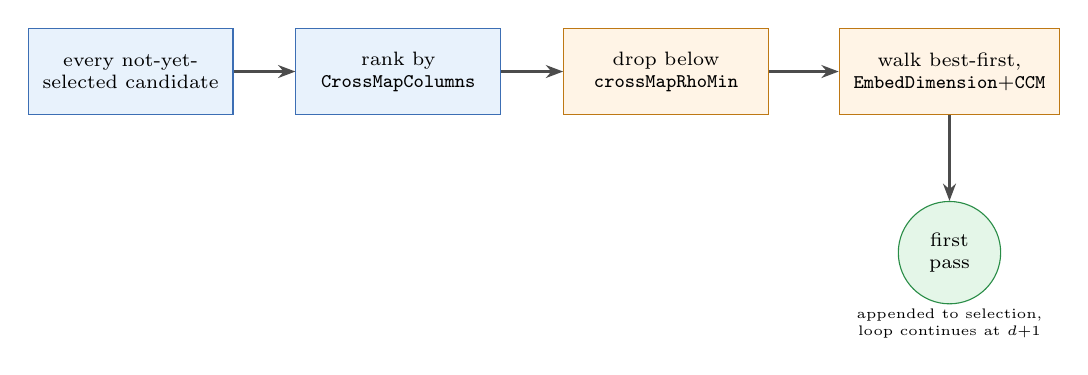
\begin{tikzpicture}[every node/.style={font=\scriptsize}]
  \node[rectangle, draw=stageline, fill=stagefill, minimum width=2.6cm, minimum height=1.1cm, align=center] (cands) at (0,0) {every not-yet-\\selected candidate};
  \node[rectangle, draw=stageline, fill=stagefill, minimum width=2.6cm, minimum height=1.1cm, align=center] (rank) at (3.4,0) {rank by\\\texttt{CrossMapColumns}};
  \node[rectangle, draw=stage2line, fill=stage2fill, minimum width=2.6cm, minimum height=1.1cm, align=center] (thresh) at (6.8,0) {drop below\\\texttt{crossMapRhoMin}};
  \node[rectangle, draw=stage2line, fill=stage2fill, minimum width=2.8cm, minimum height=1.1cm, align=center] (gate) at (10.4,0) {walk best-first,\\\texttt{EmbedDimension}+\texttt{CCM}};
  \node[circle, draw=okline, fill=okfill, minimum size=1.3cm, align=center] (accept) at (10.4,-2.3) {first\\pass};
  \draw[arrow] (cands) -- (rank);
  \draw[arrow] (rank) -- (thresh);
  \draw[arrow] (thresh) -- (gate);
  \draw[arrow] (gate) -- (accept);
  \node[font=\tiny, align=center] at (10.4,-3.2) {appended to selection,\\loop continues at $d{+}1$};
\end{tikzpicture}
\caption{One dimension of \texttt{dimx.MDE}'s forward selection: rank first (cheap), then causality-gate only the survivors, accepting the first ranked candidate that also passes CCM -- not necessarily the single best-ranked one.}
\label{fig:mde-flow}
\end{figure}

\pitfallbox{Tp matters more than its default suggests:}{\texttt{dimx.MDE}'s own unset default is \texttt{Tp=1} -- drivers get selected purely for 1-step-ahead skill, with nothing in the selection rewarding stability over a long recursive \texttt{Generate()} run. \texttt{MDE\_GMN\_TP} exposes this as a first-class parameter for exactly that reason (a driver that predicts one step ahead well can still be a poor choice for a network meant to free-run for hundreds of steps).}

\subsection{The exclusion-radius monkeypatch}
\label{sec:exclusion-radius}
The classic Theiler-window guideline is $\texttt{exclusionRadius} \ge E \times \tau$ -- but this pipeline's embeddings are generalized (Section~\ref{sec:stage2}), so $E$ and $\tau$ are confounded rather than fixed scalars: a single static bound computed once upfront cannot track an embedding that grows dimension-by-dimension across \texttt{dimx.Run()}'s own forward-selection loop, with each dimension potentially carrying a different delay. \texttt{MDE\_GMN\_EXCLUSION\_RADIUS='auto'} (default) fixes this by intercepting \texttt{dimx.Run}'s own module-level \texttt{CrossMapColumns}/\texttt{EmbedDimension}/\texttt{CCM} bindings (\texttt{\_auto\_exclusion\_radius\_cross\_map\_columns()} etc.) and recomputing \texttt{exclusionRadius} fresh, at \emph{every} call, from whichever columns that specific call is actually evaluating (dimension $\times$ largest delay among them) -- see \texttt{\_dynamic\_exclusion\_radius()}'s own docstring for the full mechanics. Setting an explicit integer instead falls back to \texttt{dimx.MDE}'s ordinary fixed-radius behavior.

\begin{figure}[H]
\centering
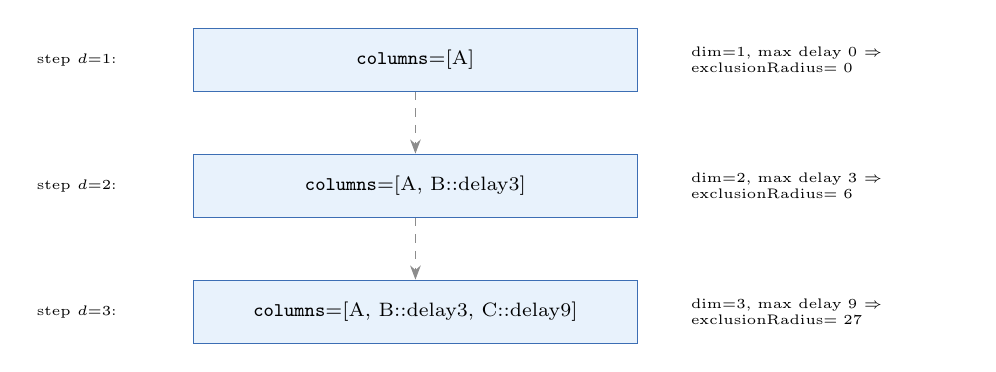
\begin{tikzpicture}[every node/.style={font=\scriptsize}]
  \foreach \d/\y/\lab/\note in {
    1/2.6/{[A]}/{dim=1, max delay 0 $\Rightarrow$ exclusionRadius$=0$},
    2/1.0/{[A, B::delay3]}/{dim=2, max delay 3 $\Rightarrow$ exclusionRadius$=6$},
    3/-0.6/{[A, B::delay3, C::delay9]}/{dim=3, max delay 9 $\Rightarrow$ exclusionRadius$=27$}
  } {
    \node[font=\tiny] at (-0.9,\y) {step $d{=}\d$:};
    \node[rectangle, draw=stageline, fill=stagefill, minimum height=0.8cm, text width=5.4cm, align=center] (n\d) at (3.4,\y) {\texttt{columns}=\lab};
    \node[font=\tiny, align=left, text width=3.4cm] at (8.6,\y) {\note};
  }
  \draw[faintarrow] (n1) -- (n2);
  \draw[faintarrow] (n2) -- (n3);
\end{tikzpicture}
\caption{\texttt{\_dynamic\_exclusion\_radius()} recomputed at every one of \texttt{dimx.Run()}'s internal calls: as forward selection accepts more (and possibly deeper-delayed) columns, the Theiler window grows to match the embedding actually in play at that exact step -- never a single worst-case bound fixed up front.}
\label{fig:exclusion-radius}
\end{figure}

\newpage
% =====================================================================
\section{GMN Simulation via a Generalized S-map Embedding}
\label{sec:smap}
% =====================================================================

\subsection{Why gmn's own \texttt{Embed()} call had to be replaced}
\texttt{gmn.GMN} simulates every node with S-map, and its installed S-map branch calls \texttt{pyEDM.Embed(E, tau, columns)} -- one shared, uniform lag applied to every predictor. That is exactly what Stages 1--2 deliberately do \emph{not} produce: a node's real embedding here is a list of (column, delay) pairs, potentially a different delay for every one. This pipeline monkeypatches \texttt{gmn.Node.\_\_init\_\_}, \texttt{gmn.Node.Forecast}, and \texttt{gmn.Node.Generate} to replace that call with its own \texttt{\_generalized\_embed()}, built directly from the graph.

\begin{figure}[H]
\centering
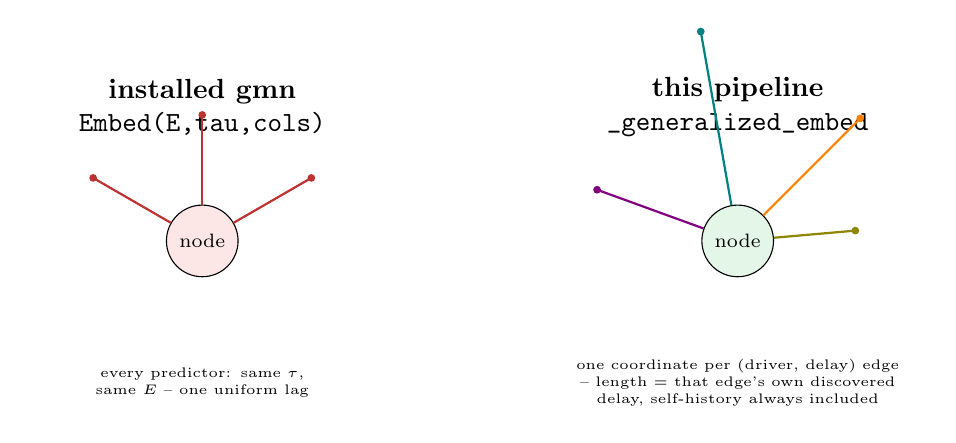
\begin{tikzpicture}[every node/.style={font=\scriptsize}]
  \node[font=\bfseries, align=center, text width=4.2cm] at (0.8,3.1) {installed gmn\\\texttt{Embed(E,tau,cols)}};
  \node[circle, draw, fill=badfill, minimum size=8mm] (nodeL) at (0.8,1.4) {node};
  \foreach \i/\a in {1/150,2/90,3/30}
    { \coordinate (pL\i) at ($(nodeL)+({\a}:1.6cm)$);
      \draw[badline, thick] (pL\i) -- (nodeL);
      \fill[badline] (pL\i) circle (1.4pt); }
  \node[font=\tiny, align=center, text width=3.6cm] at (0.8,-0.4) {every predictor: same $\tau$, same $E$ -- one uniform lag};

  \node[font=\bfseries, align=center, text width=4.6cm] at (7.6,3.1) {this pipeline\\\texttt{\_generalized\_embed}};
  \node[circle, draw, fill=okfill, minimum size=8mm] (nodeR) at (7.6,1.4) {node};
  \foreach \i/\a/\c/\len in {1/160/violet/1.3, 2/100/teal/2.1, 3/45/orange/1.6, 4/5/olive/0.9}
    { \coordinate (pR\i) at ($(nodeR)+({\a}:{\len cm+0.6cm})$);
      \draw[\c, thick] (pR\i) -- (nodeR);
      \fill[\c] (pR\i) circle (1.4pt); }
  \node[font=\tiny, align=center, text width=4.4cm] at (7.6,-0.4) {one coordinate per (driver, delay) edge -- length = that edge's own discovered delay, self-history always included};
\end{tikzpicture}
\caption{The embedding this patch replaces (left, one shared $(E,\tau)$ for every predictor) vs.\ what Stages 1--2 actually discovered (right, a genuinely non-uniform, per-driver-delay embedding) -- edge length here is schematic for "delay magnitude," not to scale.}
\label{fig:embed-comparison}
\end{figure}

\subsection{Algorithm: \texttt{\_embedding\_spec\_for} -- one node's embedding, from the graph}
\begin{steps}
\item \textbf{\texttt{MultiDiGraph} (\texttt{MODE='MDE-GMN'}):} the node's coordinates are its own \texttt{self\_delay\_set} (always present -- Section~\ref{sec:self-delay} -- regardless of how many external drivers it has) plus one coordinate per real in-edge, at that edge's own discovered delay.
\item \textbf{Plain \texttt{DiGraph} (\texttt{MODE='GMN'}):} falls back to the original uniform scheme -- $E$ lagged copies of every predecessor plus itself, at the shared \texttt{fallback\_E}/\texttt{fallback\_tau} from that mode's own CCM grid search.
\end{steps}

\subsection{Algorithm: \texttt{\_generalized\_embed}}
Builds one column per (col, delay) pair in the spec, named \texttt{col(t-k)} (matching \texttt{pyEDM.Embed()}'s own naming convention so downstream code that looks up \texttt{target(t-0)} keeps working unchanged), each holding that column's value $|{\rm delay}|$ rows in the past. Returns the embedded frame with its leading (now-NaN, now-dropped) rows removed, plus \texttt{offset} -- the largest lag magnitude in the spec -- for callers that need to realign a time column.

\begin{notebox}{Self-history is unconditional, not something Stages 1--2 have to discover.\label{sec:self-delay}}
\texttt{graph.graph['self\_delay\_set']} (set once in \texttt{build\_network()}, always \texttt{sorted(set(lag\_set) $\cup$ \{0\}}, reverse=True\texttt{)}) is unioned into \emph{every} node's embedding spec regardless of what either MDE stage found for that node's external drivers. This is why a node reached only via a single delay$\ne$0 edge (Section~\ref{sec:stage1}'s decision box) still simulates correctly: it always has its own present value plus its own lag history as fallback coordinates, the same guarantee every driverless leaf node already relied on before this generalized-embedding feature existed.
\end{notebox}

\begin{notebox}{Two pre-existing \texttt{gmn} bugs, fixed as a side effect of this same patch:}
(1) \texttt{gmn/Forecast.py} calls \texttt{Embed()} without ever importing \texttt{pyEDM.Embed} in that module (confirmed: the sibling \texttt{Generate.py} module imports it correctly; \texttt{Forecast.py} does not) -- raised \texttt{NameError} on the first S-map \texttt{Forecast()} call. Moot now that this branch no longer calls \texttt{pyEDM}'s \texttt{Embed()} at all. (2) \texttt{Forecast()}'s divergence check was \texttt{val.max() > 1E15} where \texttt{val} is a 2-tuple \texttt{(time, predictions)} -- tuples have no \texttt{.max()}, so this raised \texttt{AttributeError} \emph{unconditionally}, not only on genuine divergence. Fixed to check the predictions Series directly (\texttt{val[1]}). Every other \texttt{FunctionType} branch (Simplex, kedmSimplex, Linear, SVR, knn) is copied verbatim from the installed package, unused here since every node in this pipeline is S-map, but kept intact so the patch cannot silently change behavior for a future non-S-map code path.
\end{notebox}

\linknote{\texttt{gmn.GMN} can now simulate this pipeline's genuinely non-uniform network at \emph{any} choice of per-node theta. Nothing so far has decided which theta is best -- that's the search, Section~\ref{sec:search}.}

\newpage
% =====================================================================
\section{Hyperparameter Search: Theta and the Generate() Start Row}
\label{sec:search}
% =====================================================================

\subsection{Why this search is smaller than the sibling's}
The sibling pipeline (and this pipeline's own pre-two-stage predecessor, \texttt{scripts/backup/simple-mde-gmn\_pre-delay-embedding.py}, kept for comparison per explicit direction) searches a full $(E,\tau,\theta)$ grid, because $E$ and $\tau$ are otherwise unknowns. In this pipeline, $E$ and every driver's delay are no longer search parameters at all -- they come directly from Stages 1--2's own discovered graph (Section~\ref{sec:smap}). There is nothing left to grid-search except $\theta$, S-map's own localization parameter -- a genuine reduction in search cost, not a relocation of it: the old search's dominant cost (\texttt{len(E)} $\times$ \texttt{len(tau)} full \texttt{Generate()} calls) becomes one \texttt{Generate()} call per network.

\begin{figure}[H]
\centering
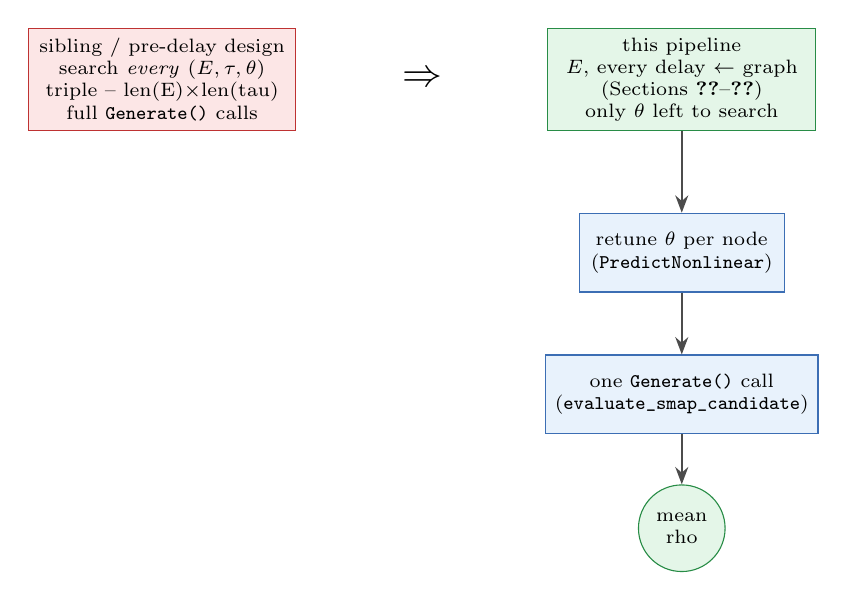
\begin{tikzpicture}[every node/.style={font=\scriptsize}]
  \node[rectangle, draw=badline, fill=badfill, minimum width=3.4cm, minimum height=1.3cm, align=center] (old) at (0,0) {sibling / pre-delay design\\search \emph{every} $(E,\tau,\theta)$\\triple -- len(E)$\times$len(tau)\\full \texttt{Generate()} calls};
  \node[rectangle, draw=okline, fill=okfill, minimum width=3.4cm, minimum height=1.3cm, align=center] (new) at (6.6,0) {this pipeline\\$E$, every delay $\leftarrow$ graph\\(Sections~\ref{sec:stage1}--\ref{sec:stage2})\\only $\theta$ left to search};
  \node[font=\Large] at (3.3,0) {$\Rightarrow$};
  \node[rectangle, draw=stageline, fill=stagefill, minimum width=2.6cm, minimum height=1cm, align=center] (retune) at (6.6,-2.2) {retune $\theta$ per node\\(\texttt{PredictNonlinear})};
  \node[rectangle, draw=stageline, fill=stagefill, minimum width=2.6cm, minimum height=1cm, align=center] (gen) at (6.6,-4.0) {one \texttt{Generate()} call\\(\texttt{evaluate\_smap\_candidate})};
  \node[circle, draw=okline, fill=okfill, minimum size=1.1cm, align=center] (score) at (6.6,-5.7) {mean\\rho};
  \draw[arrow] (new) -- (retune);
  \draw[arrow] (retune) -- (gen);
  \draw[arrow] (gen) -- (score);
\end{tikzpicture}
\caption{What the search used to cost (left) vs.\ what it costs now (right): a full grid collapses to one retune-then-score loop per network, since $E$ and every driver's delay are no longer unknowns.}
\label{fig:search-reduction}
\end{figure}

\subsection{Algorithm: \texttt{retune\_theta\_for\_all\_nodes}}
For every node, build its generalized embedding directly (not through a live \texttt{gmn.Node} -- this runs before any \texttt{gmn.GMN} object exists), split 70/30, and run \texttt{pyEDM.PredictNonlinear} over \texttt{THETA\_RANGE} to find the rho-maximizing $\theta$. Falls back to $\theta=3$ whenever there's too little data for a meaningful split (fewer than 20 prediction rows) or \texttt{PredictNonlinear} itself fails, rather than letting one bad node abort retuning for the whole network.

\pitfallbox{No TSLS-aware equivalent exists here either (same gap as the sibling, Section~\ref{sec:sibling}):}{\texttt{PredictNonlinear} scores purely by \texttt{pyEDM}'s own internal Pearson-rho criterion. Since this pipeline never TSLS-converts its inputs in the first place (Section~\ref{sec:sibling}), this is consistent with the rest of the pipeline's scoring -- but it does mean theta selection has no notion of "does this preserve spike-timing structure," only "does this maximize linear-after-local-weighting predictive skill."}

\subsection{Algorithm: \texttt{run\_theta\_search} and \texttt{evaluate\_smap\_candidate}}
Retunes theta (above), then scores the result with exactly one \texttt{Generate()} call via \texttt{evaluate\_smap\_candidate()} -- mean rho across \emph{targets only} (not driver nodes), between the simulated and real held-out series, starting at \texttt{GENERATE\_VALIDATION\_START} (never \texttt{PREDICTION\_START} -- Section~\ref{sec:split}'s leakage guard applies here too). Guarded with try/except: \texttt{gmn.Generate()} can raise \texttt{RuntimeError} on SMap divergence ($>10^{15}$) even at a retuned theta on a large network, which is a real, expected outcome for at least some configurations, not a bug to crash the whole search over.

\subsection{Algorithm: \texttt{sweep\_generate\_start}}
\texttt{Generate()} is a recursive nonlinear simulation, so which row it launches from can change how well it tracks reality, independent of how good the embedding/theta are. This sweep tries \texttt{GENERATE\_START\_MIN/MAX/STEP\_OFFSET} candidate offsets from \texttt{GENERATE\_VALIDATION\_START} (never before it -- offsets are always $\ge 0$), scores each with the same \texttt{evaluate\_smap\_candidate()} objective, and keeps the best. A single-offset default (\texttt{MIN=0, MAX=1}) disables the sweep entirely -- \texttt{rebuild\_at\_best\_params()} is about to run \texttt{Generate()} at that exact configuration anyway, so running it again here first would be a wasted duplicate call. Figure~\ref{fig:start-sweep} (Section~\ref{sec:outputs}) is a real sweep from a completed run.

\begin{figure}[H]
\centering
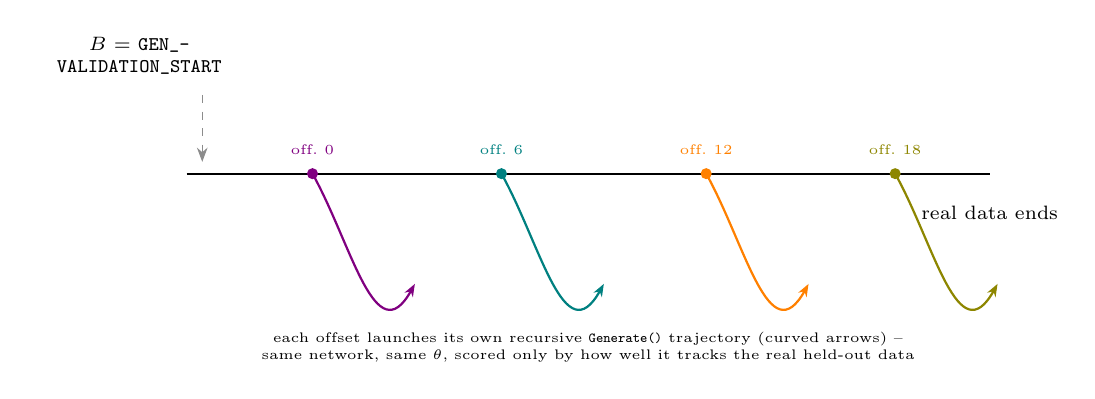
\begin{tikzpicture}[every node/.style={font=\scriptsize}]
  \draw[thick] (0,0) -- (10.2,0);
  \node[align=center, text width=2.6cm] at (-0.6,1.5) {$B$ = \texttt{GEN\_VALIDATION\_START}};
  \draw[faintarrow] (0.2,1.0) -- (0.2,0.15);
  \node[align=center] at (10.2,-0.5) {real data ends};
  \foreach \x/\c/\lab in {1.6/violet/{off.\ 0}, 4.0/teal/{off.\ 6}, 6.6/orange/{off.\ 12}, 9.0/olive/{off.\ 18}} {
    \fill[\c] (\x,0) circle (2pt);
    \draw[\c, thick, -{Stealth[length=1.6mm]}] (\x,0) .. controls +(0.5,-0.9) and +(-0.5,-0.9) .. (\x+1.3,-1.4);
    \node[font=\tiny, \c] at (\x,0.3) {\lab};
  }
  \node[font=\tiny, align=center, text width=8.6cm] at (5.1,-2.2) {each offset launches its own recursive \texttt{Generate()} trajectory (curved arrows) -- same network, same $\theta$, scored only by how well it tracks the real held-out data};
\end{tikzpicture}
\caption{The start-point sweep, schematically: the identical model, launched from several different rows within $[B,\mathrm{end})$, can track reality very differently -- Figure~\ref{fig:start-sweep} (Section~\ref{sec:outputs}) shows this is not just a theoretical concern on real data.}
\label{fig:start-sweep-schematic}
\end{figure}

\pitfallbox{Checkpointing here is intra-job only, unlike the cross-job cache (Section~\ref{sec:storage}):}{\texttt{sweep\_generate\_start()} writes a pickle checkpoint to \texttt{results\_dir} after every offset so a job that dies mid-sweep can resume \emph{within the same submission}. The cross-job fingerprinted cache (\texttt{reuse\_cache}/\texttt{RUN\_CACHE\_DIR}) is a separate, additional mechanism that lets a full resubmission after a crash skip the whole sweep -- see Section~\ref{sec:storage} for why both exist.}

\newpage
% =====================================================================
\section{Final Validation}
\label{sec:validation}
% =====================================================================
Three independent diagnostics, deliberately not collapsed into one number, so a network that looks good on one metric but not another is visible rather than averaged away.

\begin{figure}[H]
\centering
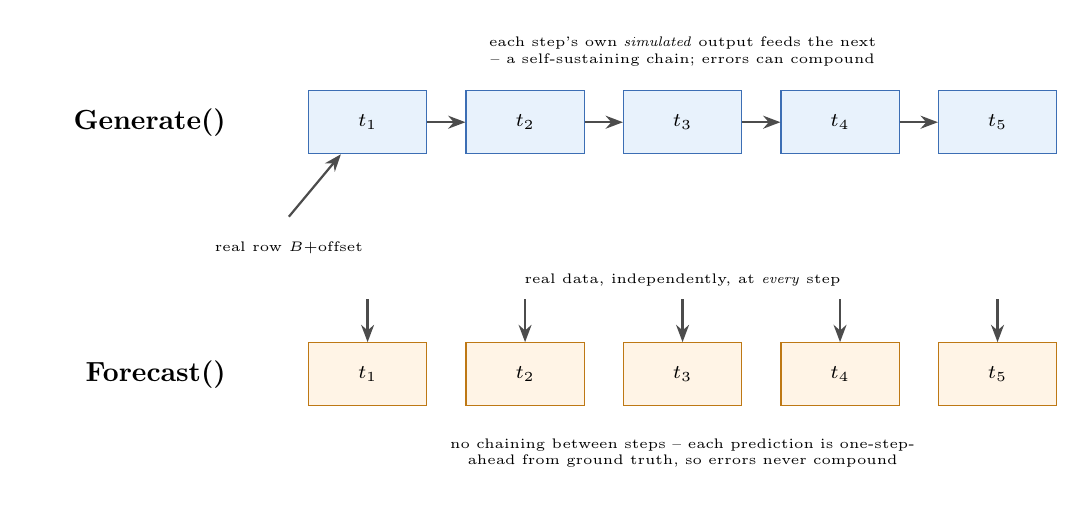
\begin{tikzpicture}[every node/.style={font=\scriptsize}]
  \node[align=right, font=\bfseries, text width=2.4cm] at (-3.0,2.2) {Generate()};
  \foreach \i/\x in {1/0,2/2,3/4,4/6,5/8}
    \node[rectangle, draw=stageline, fill=stagefill, minimum width=1.5cm, minimum height=0.8cm] (g\i) at (\x,2.2) {$t_{\i}$};
  \draw[arrow] (-1.0,1.0) -- (g1);
  \node[font=\tiny] at (-1.0,0.6) {real row $B{+}$offset};
  \foreach \i/\j in {1/2,2/3,3/4,4/5} \draw[arrow] (g\i) -- (g\j);
  \node[font=\tiny, text width=8.6cm, align=center] at (4,3.1) {each step's own \emph{simulated} output feeds the next -- a self-sustaining chain; errors can compound};

  \node[align=right, font=\bfseries, text width=2.4cm] at (-3.0,-1.0) {Forecast()};
  \foreach \i/\x in {1/0,2/2,3/4,4/6,5/8}
    \node[rectangle, draw=stage2line, fill=stage2fill, minimum width=1.5cm, minimum height=0.8cm] (f\i) at (\x,-1.0) {$t_{\i}$};
  \foreach \i/\x in {1/0,2/2,3/4,4/6,5/8}
    \draw[arrow] (\x,-0.05) -- (f\i);
  \node[font=\tiny] at (4,0.2) {real data, independently, at \emph{every} step};
  \node[font=\tiny, text width=8.6cm, align=center] at (4,-2.0) {no chaining between steps -- each prediction is one-step-ahead from ground truth, so errors never compound};
\end{tikzpicture}
\caption{Why both diagnostics matter: \texttt{Generate()} tests whether the network can sustain itself free-running (Section~\ref{sec:validation}'s "accumulation problem"); \texttt{Forecast()} tests one-step skill in isolation, with real data reinjected at every step. A network can score well on one and poorly on the other.}
\label{fig:generate-vs-forecast}
\end{figure}

\subsection{Algorithm: \texttt{rebuild\_at\_best\_params}}
Reruns \texttt{Generate()} once more at the search's winning theta and start row (needed downstream regardless, since the search's own probe \texttt{Generate()} calls aren't retained). Guarded per-network: a divergence here is logged and that network is skipped (\texttt{run['G']} stays unset) rather than crashing the whole job and losing every other network's already-finished work.

\subsection{Algorithm: \texttt{run\_forecast\_diagnostic}}
Runs \texttt{Forecast()} (one-step-ahead, using the \emph{real} data at every step, not the network's own prior output) at the same winning parameters, and plots it alongside the free-running \texttt{Generate()} trace and the real data (Figure~\ref{fig:generate-forecast}). This separates two failure modes: a network that forecasts well one step ahead but diverges when run freely has an \emph{accumulation} problem, not a one-step prediction problem.

\subsection{Algorithm: \texttt{gmn\_fidelity\_rho}}
For every node: build a two-column (simulated, real) table at matching time indices, run a Simplex prediction of "real" from "simulated," and score it. This is a Fig-4e-style generative fidelity check (matching the source literature's own construction for this kind of network): it asks not "did the curves look similar" but "does the simulated trajectory's own internal dynamics let you recover the real one" -- a stricter, structure-aware question than raw correlation between the two curves. Figure~\ref{fig:fidelity} (Section~\ref{sec:outputs}) is real output from this exact function.

\begin{figure}[H]
\centering
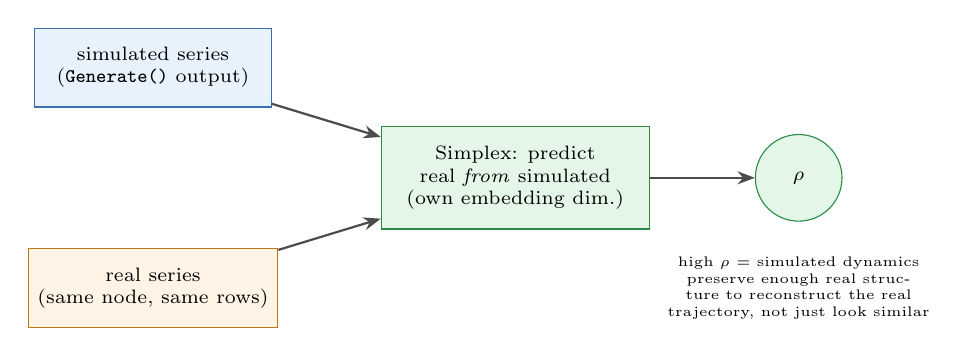
\begin{tikzpicture}[every node/.style={font=\scriptsize}]
  \node[rectangle, draw=stageline, fill=stagefill, minimum width=3cm, minimum height=1cm, align=center] (sim) at (0,1.4) {simulated series\\(\texttt{Generate()} output)};
  \node[rectangle, draw=stage2line, fill=stage2fill, minimum width=3cm, minimum height=1cm, align=center] (real) at (0,-1.4) {real series\\(same node, same rows)};
  \node[rectangle, draw=okline, fill=okfill, minimum width=3.4cm, minimum height=1.3cm, align=center] (simplex) at (4.6,0) {Simplex: predict\\real \emph{from} simulated\\(own embedding dim.)};
  \draw[arrow] (sim) -- (simplex);
  \draw[arrow] (real) -- (simplex);
  \node[circle, draw=okline, fill=okfill, minimum size=1.1cm] (rho) at (8.2,0) {$\rho$};
  \draw[arrow] (simplex) -- (rho);
  \node[font=\tiny, text width=3.6cm, align=center] at (8.2,-1.4) {high $\rho$ = simulated dynamics preserve enough real structure to reconstruct the real trajectory, not just look similar};
\end{tikzpicture}
\caption{The Fig-4e-style fidelity metric: a structure-aware test (can you recover reality \emph{from} the simulation's own internal geometry), stricter than a plain correlation between the two curves.}
\label{fig:fidelity-schematic}
\end{figure}

\linknote{These three diagnostics are the pipeline's actual deliverable. Section~\ref{sec:outputs} shows what they produced on the most recent completed run of this exact codebase.}

\newpage
% =====================================================================
\section{Stage 6: MDE-only Diagnostics}
\label{sec:diagnostics}
% =====================================================================
(Skipped when \texttt{MODE='GMN}'; controlled by \texttt{RUN\_MDE\_DIAGNOSTICS} otherwise.)

\subsection{\texttt{run\_mde\_evaluate}}
For each target, compares \texttt{dimx.Evaluate}'s reconstruction-quality metrics (CAE, RMSE, R, $R^2$) for MDE's own selection against two unsupervised baselines -- PCA and diffusion-map embeddings of the same candidate pool. Unlike the sibling pipeline (which dropped this diagnostic outright when it ported away from \texttt{dimx.MDE}'s own result object, sibling Section~6), this pipeline still uses \texttt{dimx.MDE} natively, so this comparison remains available -- see Section~\ref{sec:outputs} for a real result.

\begin{figure}[H]
\centering
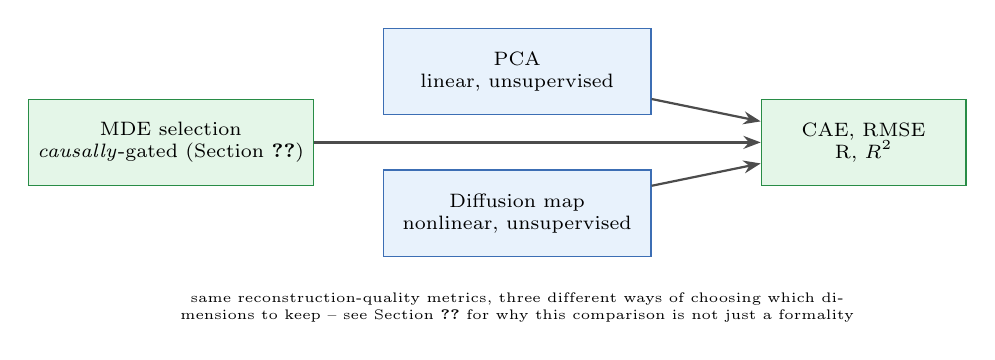
\begin{tikzpicture}[every node/.style={font=\scriptsize}]
  \node[rectangle, draw=okline, fill=okfill, minimum width=3.4cm, minimum height=1.1cm, align=center] (mde) at (0,0) {MDE selection\\\emph{causally}-gated (Section~\ref{sec:dimx})};
  \node[rectangle, draw=stageline, fill=stagefill, minimum width=3.4cm, minimum height=1.1cm, align=center] (pca) at (4.4,0.9) {PCA\\linear, unsupervised};
  \node[rectangle, draw=stageline, fill=stagefill, minimum width=3.4cm, minimum height=1.1cm, align=center] (dmap) at (4.4,-0.9) {Diffusion map\\nonlinear, unsupervised};
  \node[rectangle, draw=okline, fill=okfill, minimum width=2.6cm, minimum height=1.1cm, align=center] (score) at (8.8,0) {CAE, RMSE\\R, $R^2$};
  \draw[arrow] (mde) -- (score);
  \draw[arrow] (pca) -- (score);
  \draw[arrow] (dmap) -- (score);
  \node[font=\tiny, text width=8.6cm, align=center] at (4.4,-2.1) {same reconstruction-quality metrics, three different ways of choosing which dimensions to keep -- see Section~\ref{sec:outputs} for why this comparison is not just a formality};
\end{tikzpicture}
\caption{\texttt{run\_mde\_evaluate()}'s comparison: MDE's causally-gated selection is scored on equal footing against two unsupervised baselines that know nothing about causality, only variance/manifold structure.}
\label{fig:mde-evaluate}
\end{figure}

\subsection{\texttt{run\_tp\_vs\_rho\_sweep} and \texttt{run\_univariate\_e\_tau\_grid}}
Sweep the prediction horizon $T_p$ using each target's MDE-selected columns as a fixed embedding (predictability-horizon diagnostic), and a univariate self-prediction $(E,\tau)$ grid per target (independent of Stages 1--2's own graph-derived embeddings), heatmapped with any cell above \texttt{GRID\_RHO\_THRESHOLD} boxed.

\begin{figure}[H]
\centering
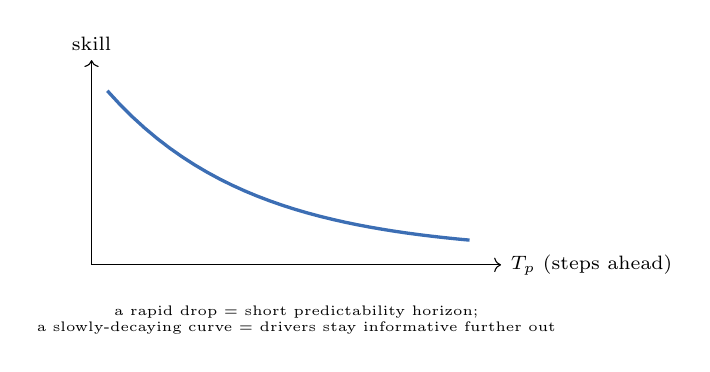
\begin{tikzpicture}[every node/.style={font=\scriptsize}]
  \draw[->] (0,0) -- (5.2,0) node[right] {$T_p$ (steps ahead)};
  \draw[->] (0,0) -- (0,2.6) node[above] {skill};
  \draw[stageline, very thick, domain=0.2:4.8, samples=30] plot ({\x}, {2.3*exp(-0.55*\x)+0.15});
  \node[font=\tiny, align=center] at (2.6,-0.7) {a rapid drop = short predictability horizon;\\a slowly-decaying curve = drivers stay informative further out};
\end{tikzpicture}
\caption{\texttt{run\_tp\_vs\_rho\_sweep}, schematically: how far into the future a target's MDE-selected drivers remain informative, independent of the network's own \texttt{Generate()} fidelity.}
\label{fig:tp-sweep-schematic}
\end{figure}

\newpage
% =====================================================================
\section{Cross-Job Search Reuse and the Fingerprinting Architecture}
\label{sec:reuse}
% =====================================================================

\subsection{The problem: every expensive stage is deterministic, but resubmission used to redo it anyway}
MDE forward selection (Sections~\ref{sec:stage1}--\ref{sec:stage2}), network construction, theta search, and the generate-start sweep are each fully determined by their own inputs. A SLURM resubmission with identical settings -- common after a timeout on a multi-day job -- used to pay for all of them again, for no reason.

\subsection{Algorithm: fingerprint-then-lookup, at four independent granularities}
\begin{steps}
\item Each stage builds its own fingerprint (\texttt{build\_mde\_selection\_fingerprint()}, \texttt{build\_network\_fingerprint()}, \texttt{build\_search\_fingerprint()}, \texttt{build\_start\_sweep\_fingerprint()}) -- every config knob that shapes that stage's outcome, plus a hash of the input data file and a fingerprint of the pipeline's own code (\texttt{build\_code\_fingerprint()}, Section~\ref{sec:code-fingerprint}).
\item \texttt{find\_cached()} scans \texttt{MDE\_GMN\_PREV\_RUNS\_DIR} for a past job's matching cache file with an identical fingerprint.
\item A hit skips that stage's real work entirely and reconstructs its result from the cache; a miss (different settings, or the first run ever with these settings) just computes it normally -- always a safe, redundant-compute optimization, never a correctness shortcut, since a mismatch can never produce a false hit.
\end{steps}

\begin{figure}[H]
\centering
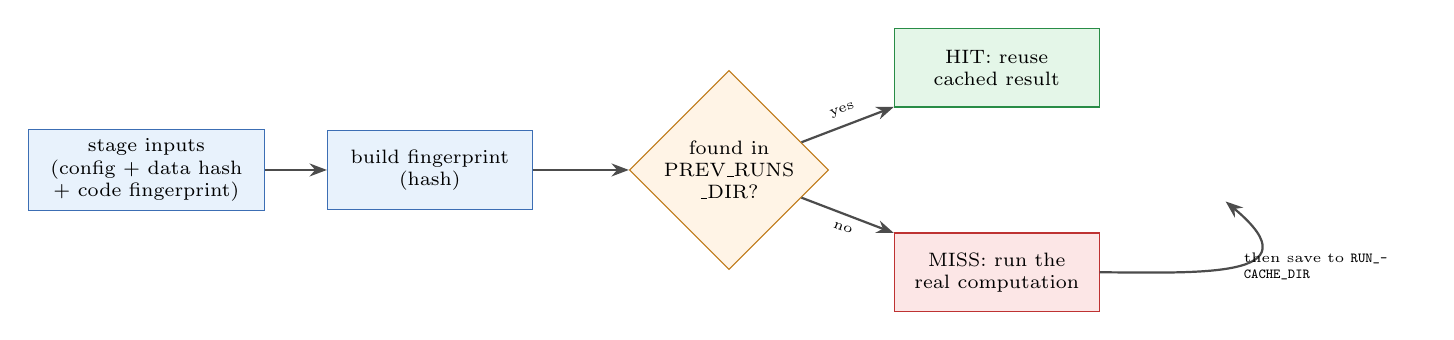
\begin{tikzpicture}[every node/.style={font=\scriptsize}]
  \node[rectangle, draw=stageline, fill=stagefill, minimum width=3cm, minimum height=1cm, align=center] (inputs) at (0,0) {stage inputs\\(config + data hash\\+ code fingerprint)};
  \node[rectangle, draw=stageline, fill=stagefill, minimum width=2.6cm, minimum height=1cm, align=center] (fp) at (3.6,0) {build fingerprint\\(hash)};
  \node[diamond, draw=stage2line, fill=stage2fill, minimum width=2.4cm, minimum height=1.6cm, align=center, inner sep=1pt] (lookup) at (7.4,0) {found in\\PREV\_RUNS\\\_DIR?};
  \node[rectangle, draw=okline, fill=okfill, minimum width=2.6cm, minimum height=1cm, align=center] (hit) at (10.8,1.3) {HIT: reuse\\cached result};
  \node[rectangle, draw=badline, fill=badfill, minimum width=2.6cm, minimum height=1cm, align=center] (miss) at (10.8,-1.3) {MISS: run the\\real computation};
  \draw[arrow] (inputs) -- (fp);
  \draw[arrow] (fp) -- (lookup);
  \draw[arrow] (lookup) -- (hit) node[midway, above, sloped, font=\tiny] {yes};
  \draw[arrow] (lookup) -- (miss) node[midway, below, sloped, font=\tiny] {no};
  \draw[arrow] (miss.east) .. controls +(1.2,0) and +(1.2,-1.0) .. ($(miss.east)+(1.6,0.9)$) node[midway, right, font=\tiny, text width=2.2cm] {then save to \texttt{RUN\_CACHE\_DIR}};
\end{tikzpicture}
\caption{The same fingerprint-then-lookup pattern, applied independently by MDE selection, network construction, theta search, and the start-point sweep -- a mismatched fingerprint can only ever fall through to MISS, never produce a false HIT.}
\label{fig:fingerprint-flow}
\end{figure}

Caching happens at full per-node granularity for MDE (Section~\ref{sec:leakage-guard}'s \texttt{run\_mde\_for\_target()} is the single call site all three MDE call sites -- \texttt{main()}'s top-level seed, Stage 1, Stage 2 -- share), so a resubmission can resume node-by-node, not just stage-by-stage.

\subsection{\texttt{build\_code\_fingerprint} -- surviving a cosmetic edit}
\label{sec:code-fingerprint}
\texttt{\_strip\_docstrings()} parses this file's own AST and removes every docstring before hashing -- so a pure documentation edit (like the one that produced most of the docstrings quoted throughout this document) does not invalidate every cache entry from every past job, while any change to actual logic still does.

\linknote{Cached artifacts need somewhere durable to live -- Section~\ref{sec:storage} covers where, and why that answer changed twice during this project's development.}

\newpage
% =====================================================================
\section{Cluster Storage Architecture}
\label{sec:storage}
% =====================================================================

\subsection{Four locations, three different lifetimes}
\begin{figure}[h]
\centering
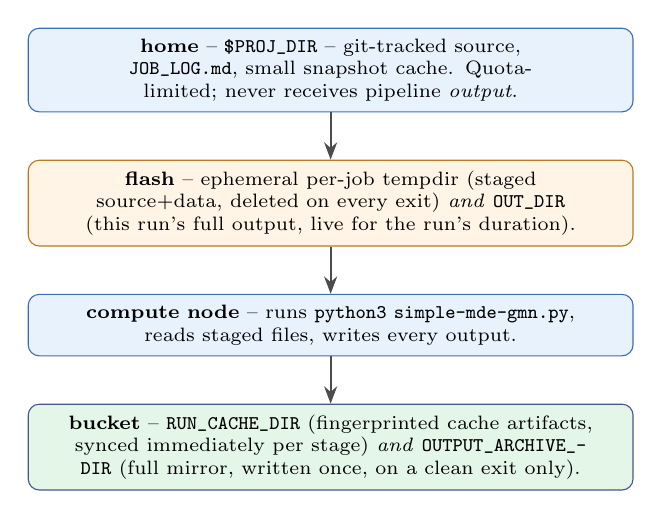
\begin{tikzpicture}[node distance=6mm, every node/.style={font=\scriptsize}]
  \node[smallbox, text width=7.4cm, draw=stageline] (home) {\textbf{home} -- \texttt{\$PROJ\_DIR} -- git-tracked source, \texttt{JOB\_LOG.md}, small snapshot cache. Quota-limited; never receives pipeline \emph{output}.};
  \node[smallbox, text width=7.4cm, below=of home, draw=flashline, fill=stage2fill] (flash) {\textbf{flash} -- ephemeral per-job tempdir (staged source+data, deleted on every exit) \emph{and} \texttt{OUT\_DIR} (this run's full output, live for the run's duration).};
  \node[smallbox, text width=7.4cm, below=of flash, draw=stageline] (compute) {\textbf{compute node} -- runs \texttt{python3 simple-mde-gmn.py}, reads staged files, writes every output.};
  \node[smallbox, text width=7.4cm, below=of compute, draw=bucketline, fill=okfill] (bucket) {\textbf{bucket} -- \texttt{RUN\_CACHE\_DIR} (fingerprinted cache artifacts, synced immediately per stage) \emph{and} \texttt{OUTPUT\_ARCHIVE\_DIR} (full mirror, written once, on a clean exit only).};
  \draw[arrow] (home) -- (flash);
  \draw[arrow] (flash) -- (compute);
  \draw[arrow] (compute) -- (bucket);
\end{tikzpicture}
\caption{The four storage locations this pipeline touches, and what each one is actually for.}
\label{fig:storage}
\end{figure}

\subsection{The job-end fork: archive on success, preserve in place on failure}
\begin{steps}
\item The sbatch script captures \texttt{python3 simple-mde-gmn.py}'s own exit status (\texttt{PY\_STATUS}) around a deliberate \texttt{set +e}/\texttt{set -e} pair -- necessary because the script otherwise runs under \texttt{set -euo pipefail}, which would jump straight to the exit trap on a nonzero exit without ever reaching the line that captures it.
\item The \texttt{cleanup} \texttt{EXIT} trap checks \texttt{PY\_STATUS}: \texttt{"0"} means the run completed cleanly, so \texttt{OUT\_DIR} is copied in full to \texttt{OUTPUT\_ARCHIVE\_DIR} (bucket) and the flash copy is then deleted.
\item Any other value -- a crash, a SLURM time-limit kill, a cancellation -- leaves \texttt{OUT\_DIR} exactly where it is on flash, untouched, for direct inspection.
\end{steps}
\decisionbox{Why this fork exists, not just "always archive" or "always keep on flash":}{Per explicit direction: flash is meant to be genuine scratch, not permanent storage, once bucket has the headroom to be the durable copy -- but a failed run's partial output is exactly the case where fast, directly-browsable storage (rather than needing to dig it out of an archive) is most useful, so failure is deliberately excluded from the archive-and-clear path.}

\pitfallbox{This fork does not apply retroactively:}{Slurm freezes a submitted job's own script content at \texttt{sbatch} time; a script that already sat queued when this fork was added to the canonical file on disk still ran with whatever it had at submission. One resubmission (job 38857309) was broken this exact way when a \emph{shared, non-frozen} script it calls by path (\texttt{generate\_job\_description.sh}) was edited while it was still queued -- see Section~\ref{sec:history-shared-script}.}

\subsection{The empty-network-directory fix}
\texttt{scripts/batch/submit.sh} used to create \texttt{\$PROJ\_DIR/results/job\_<id>/} on home and pass it to \texttt{generate\_job\_description.sh} before every job even started -- but that script only ever writes to \texttt{JOB\_LOG.md} and a small shared \texttt{.snapshots/} cache, never into a per-job directory (its own docstring: \emph{"Deliberately not a per-job copy ... every job's own .py/.sbatch content is byte-identical to either the live canonical files or fully reconstructable from JOB\_LOG.md's own diff history"}). Every submission left a permanently empty directory behind. Fixed by removing the unused parameter from \texttt{generate\_job\_description.sh} and all four of its call sites, rather than only papering over the symptom in \texttt{submit.sh}.

\newpage
% =====================================================================
\section{End-to-End Data Flow}
\label{sec:e2e}
% =====================================================================

\begin{figure}[h]
\centering
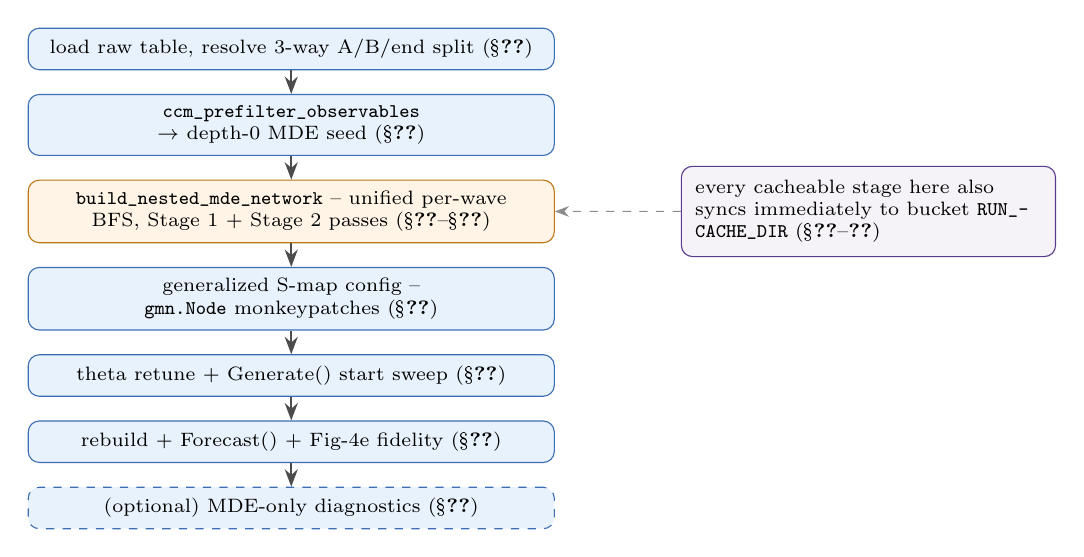
\begin{tikzpicture}[scale=0.85, every node/.style={font=\scriptsize}, node distance=3mm]
  \node[smallbox, text width=6.4cm] (load) {load raw table, resolve 3-way A/B/end split (\S\ref{sec:split})};
  \node[smallbox, text width=6.4cm, below=of load] (pre) {\texttt{ccm\_prefilter\_observables} $\to$ depth-0 MDE seed (\S\ref{sec:ccm-prefilter-section})};
  \node[smallbox, text width=6.4cm, below=of pre, fill=stage2fill, draw=stage2line] (s1) {\texttt{build\_nested\_mde\_network} -- unified per-wave BFS, Stage 1 + Stage 2 passes (\S\ref{sec:stage1}--\S\ref{sec:stage2})};
  \node[smallbox, text width=6.4cm, below=of s1] (smap) {generalized S-map config -- \texttt{gmn.Node} monkeypatches (\S\ref{sec:smap})};
  \node[smallbox, text width=6.4cm, below=of smap] (search) {theta retune + Generate() start sweep (\S\ref{sec:search})};
  \node[smallbox, text width=6.4cm, below=of search] (validate) {rebuild + Forecast() + Fig-4e fidelity (\S\ref{sec:validation})};
  \node[smallbox, text width=6.4cm, below=of validate, dashed] (diag) {(optional) MDE-only diagnostics (\S\ref{sec:diagnostics})};
  \foreach \a/\b in {load/pre,pre/s1,s1/smap,smap/search,search/validate,validate/diag}
    \draw[arrow] (\a) -- (\b);
  \node[right=1.6cm of s1, text width=4.4cm, draw=linknote, fill=linknote!6, rounded corners, inner sep=5pt] (sidenote) {every cacheable stage here also syncs immediately to bucket \texttt{RUN\_CACHE\_DIR} (\S\ref{sec:reuse}--\ref{sec:storage})};
  \draw[faintarrow] (sidenote.west) -- (s1.east);
\end{tikzpicture}
\caption{Full pipeline data flow, \texttt{main()}'s actual call order.}
\label{fig:e2e}
\end{figure}

\newpage
% =====================================================================
\section{Actual Outputs: A Real Completed Run}
\label{sec:outputs}
% =====================================================================

\subsection{What this run was, honestly}
Job 37946959 (2026-08-14, COMPLETED in 2h39m) is the most recent \emph{genuinely completed, end-to-end} run of this exact two-stage codebase. It ran at a deliberately tiny scale -- \texttt{MDE\_D=4}, \texttt{NESTED\_M=1}, \texttt{REGION\_CHANNEL\_CAP=15} (45 real observables instead of the full 468), \texttt{GENERATE\_LENGTH=20} -- so every number below should be read as \emph{"the pipeline runs correctly and produces real, if modest, results at this scale,"} not as a claim about full-scale predictive skill. The full-scale run (\texttt{MDE\_D=30}, \texttt{REGION\_CHANNEL\_CAP=999}, job 38871293) was still queued at the time of writing; Section~\ref{sec:future} covers what to check once it lands.

\subsection{What Stage 1 and Stage 2 actually built}
For \texttt{head\_position\_x}: Stage 1 built a 13-node, 14-edge real-observable backbone. Stage 2 then attached \textbf{928} lagged edges across those same 13 nodes -- growing the graph to \textbf{46 total nodes} (45 real observables plus the target itself: at this candidate-pool size, Stage 2's whole-universe search ends up touching essentially every available real observable, as at least one lagged driver for some node). Figure~\ref{fig:real-network} is the actual constructed network.

\begin{figure}[H]
\centering
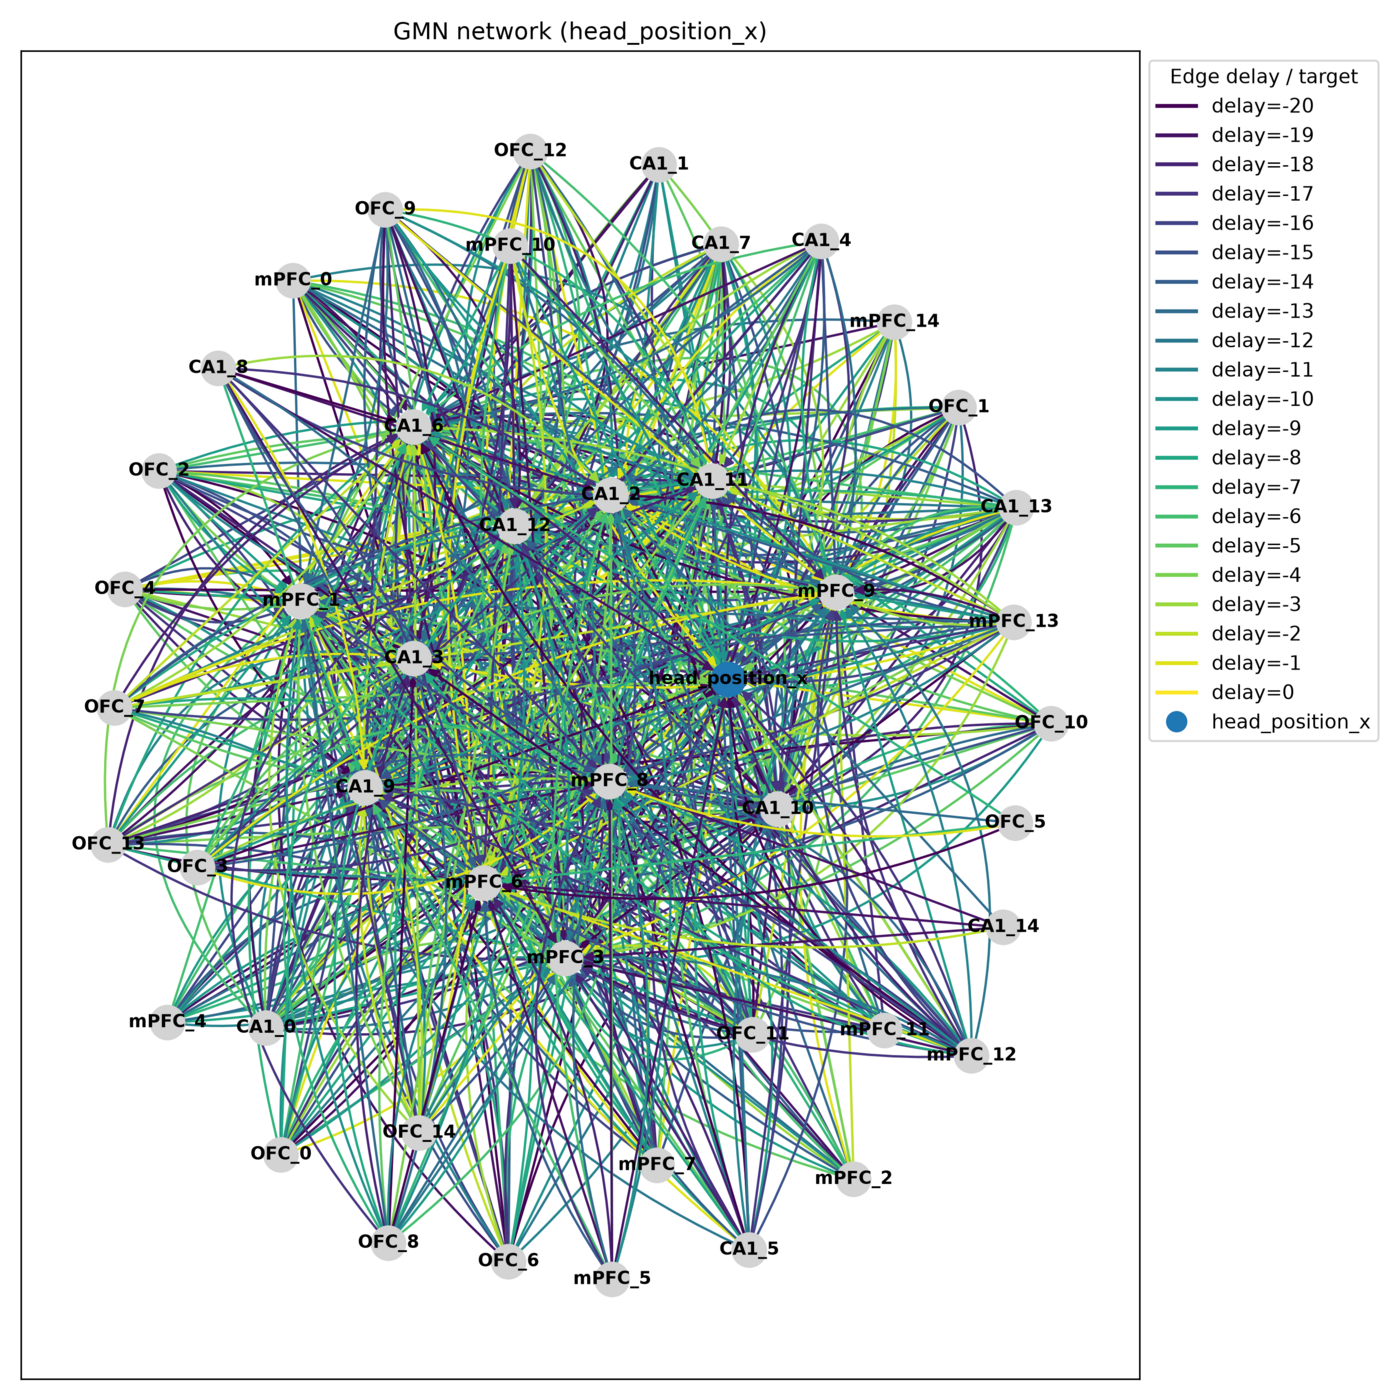
\includegraphics[width=0.82\textwidth]{figures/gmn_network_head_position_x_small.png}
\caption{The real network \texttt{draw\_colored\_network()} produced for \texttt{head\_position\_x} on job 37946959. Edge color encodes delay (legend, right) -- the dense, multi-colored fan into every node is Stage 2's lagged-embedding attachment made visible; the sparser structure among the 13 labeled hub nodes is Stage 1's backbone.}
\label{fig:real-network}
\end{figure}

\subsection{Stage 1's own selection quality}
\begin{figure}[H]
\centering
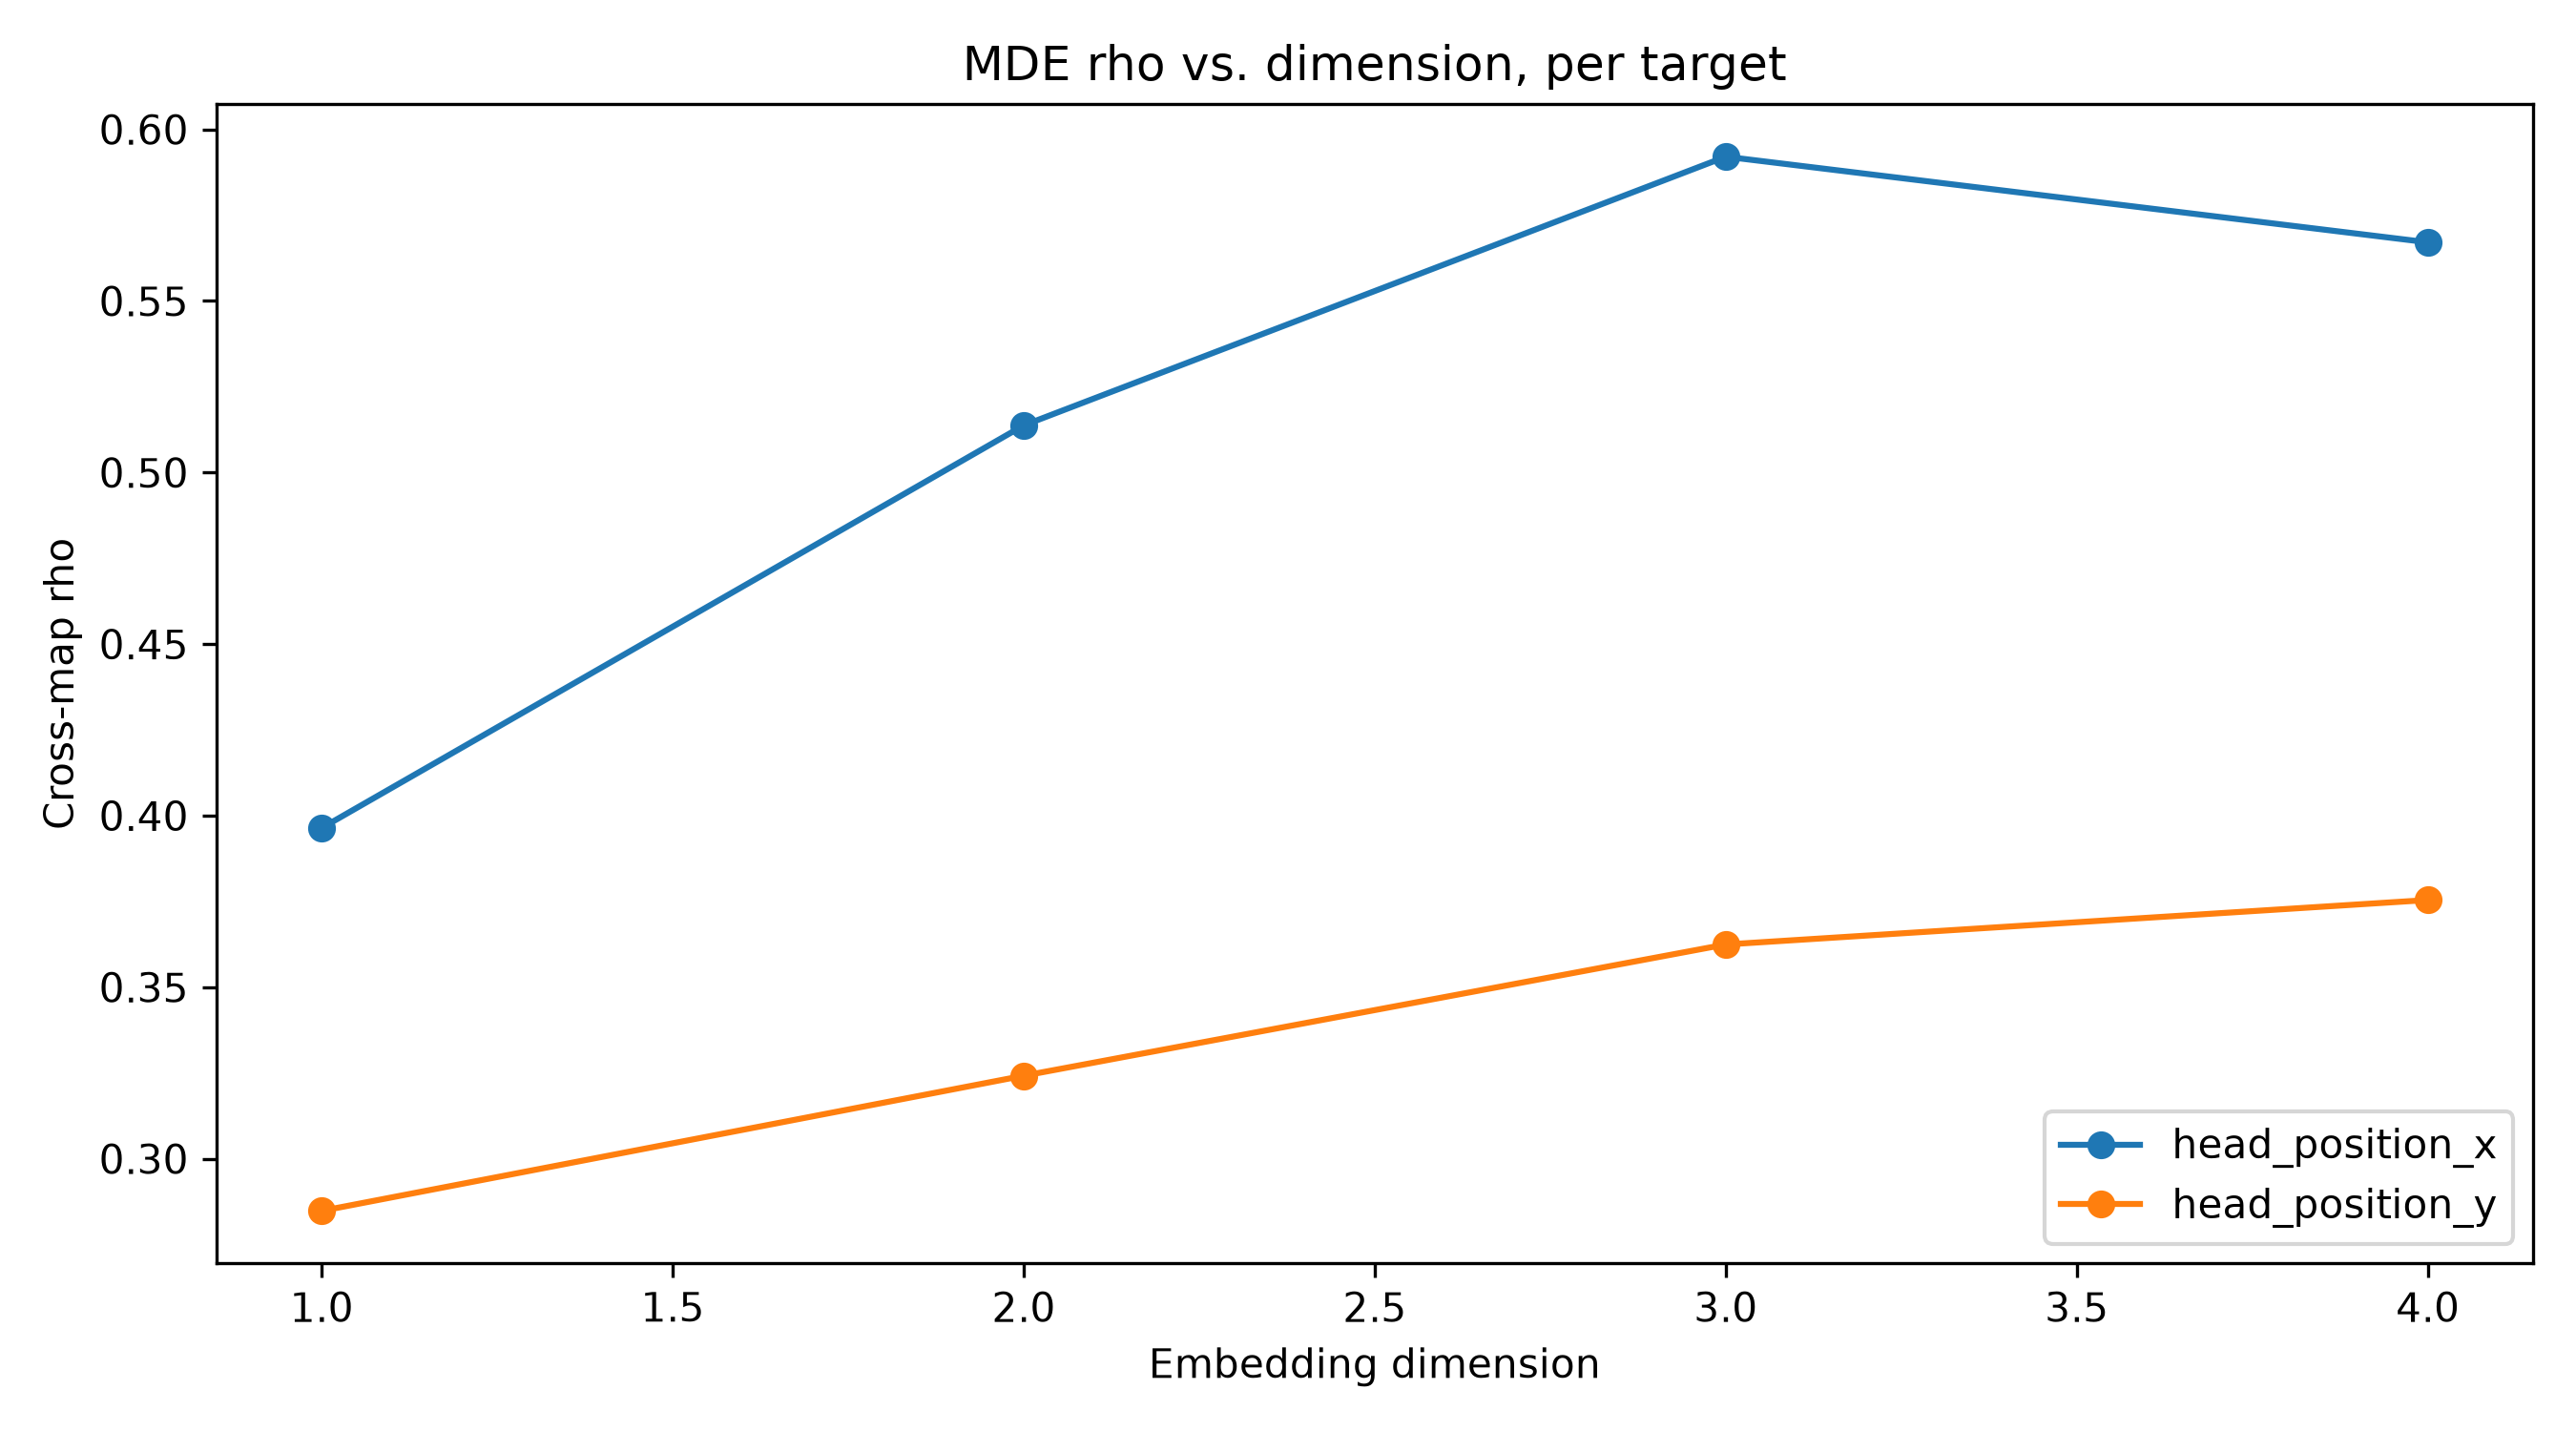
\includegraphics[width=0.78\textwidth]{figures/mde_rho_vs_dimension_multi_target.png}
\caption{Real \texttt{plot\_mde\_rho\_vs\_dimension()} output: depth-0 MDE cross-map rho as each target's forward selection adds its 1st through 4th driver. Both targets show the expected diminishing-but-positive-returns shape; \texttt{head\_position\_x} reaches a noticeably higher ceiling ($\approx$0.59) than \texttt{head\_position\_y} ($\approx$0.38) at this channel cap.}
\label{fig:rho-vs-dim}
\end{figure}

\subsection{Generative fidelity (Fig-4e-style)}
\begin{figure}[H]
\centering
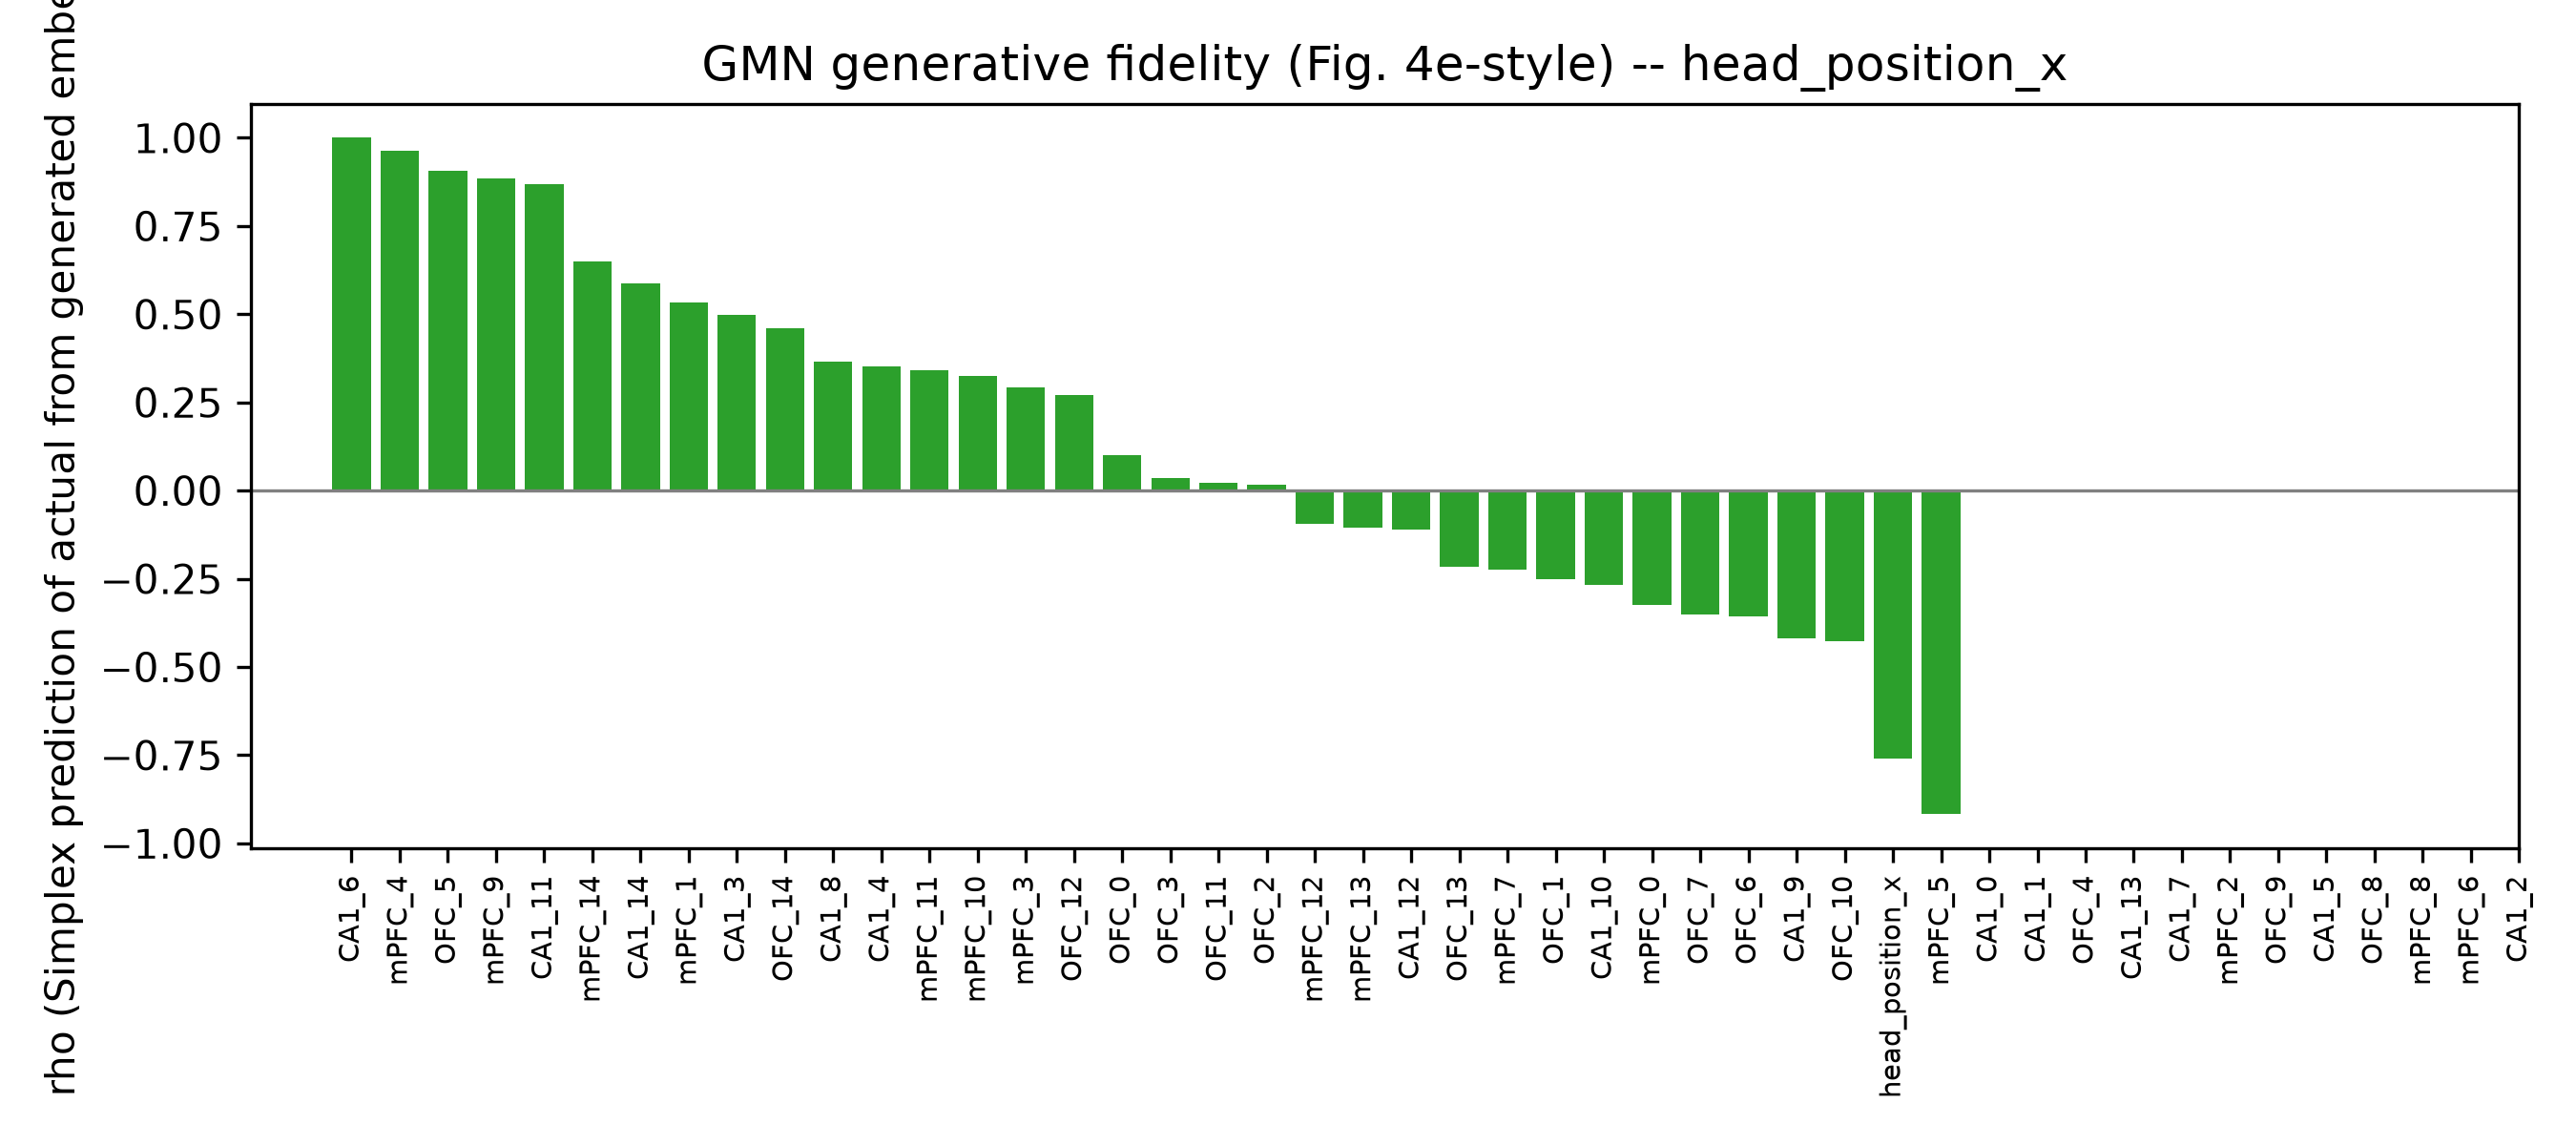
\includegraphics[width=0.82\textwidth]{figures/gmn_fidelity_head_position_x.png}
\caption{Real \texttt{gmn\_fidelity\_rho()} / \texttt{plot\_fidelity()} output for \texttt{head\_position\_x}'s network. Several driver nodes (CA1\_6, mPFC\_4, OFC\_5, mPFC\_9, CA1\_11) show strong fidelity ($\rho>0.85$); the target itself and a handful of nodes fall negative -- exactly the kind of per-node spread the Fig-4e-style diagnostic is designed to surface rather than average away (Section~\ref{sec:validation}).}
\label{fig:fidelity}
\end{figure}

\subsection{Generate() start-point sensitivity}
\begin{figure}[H]
\centering
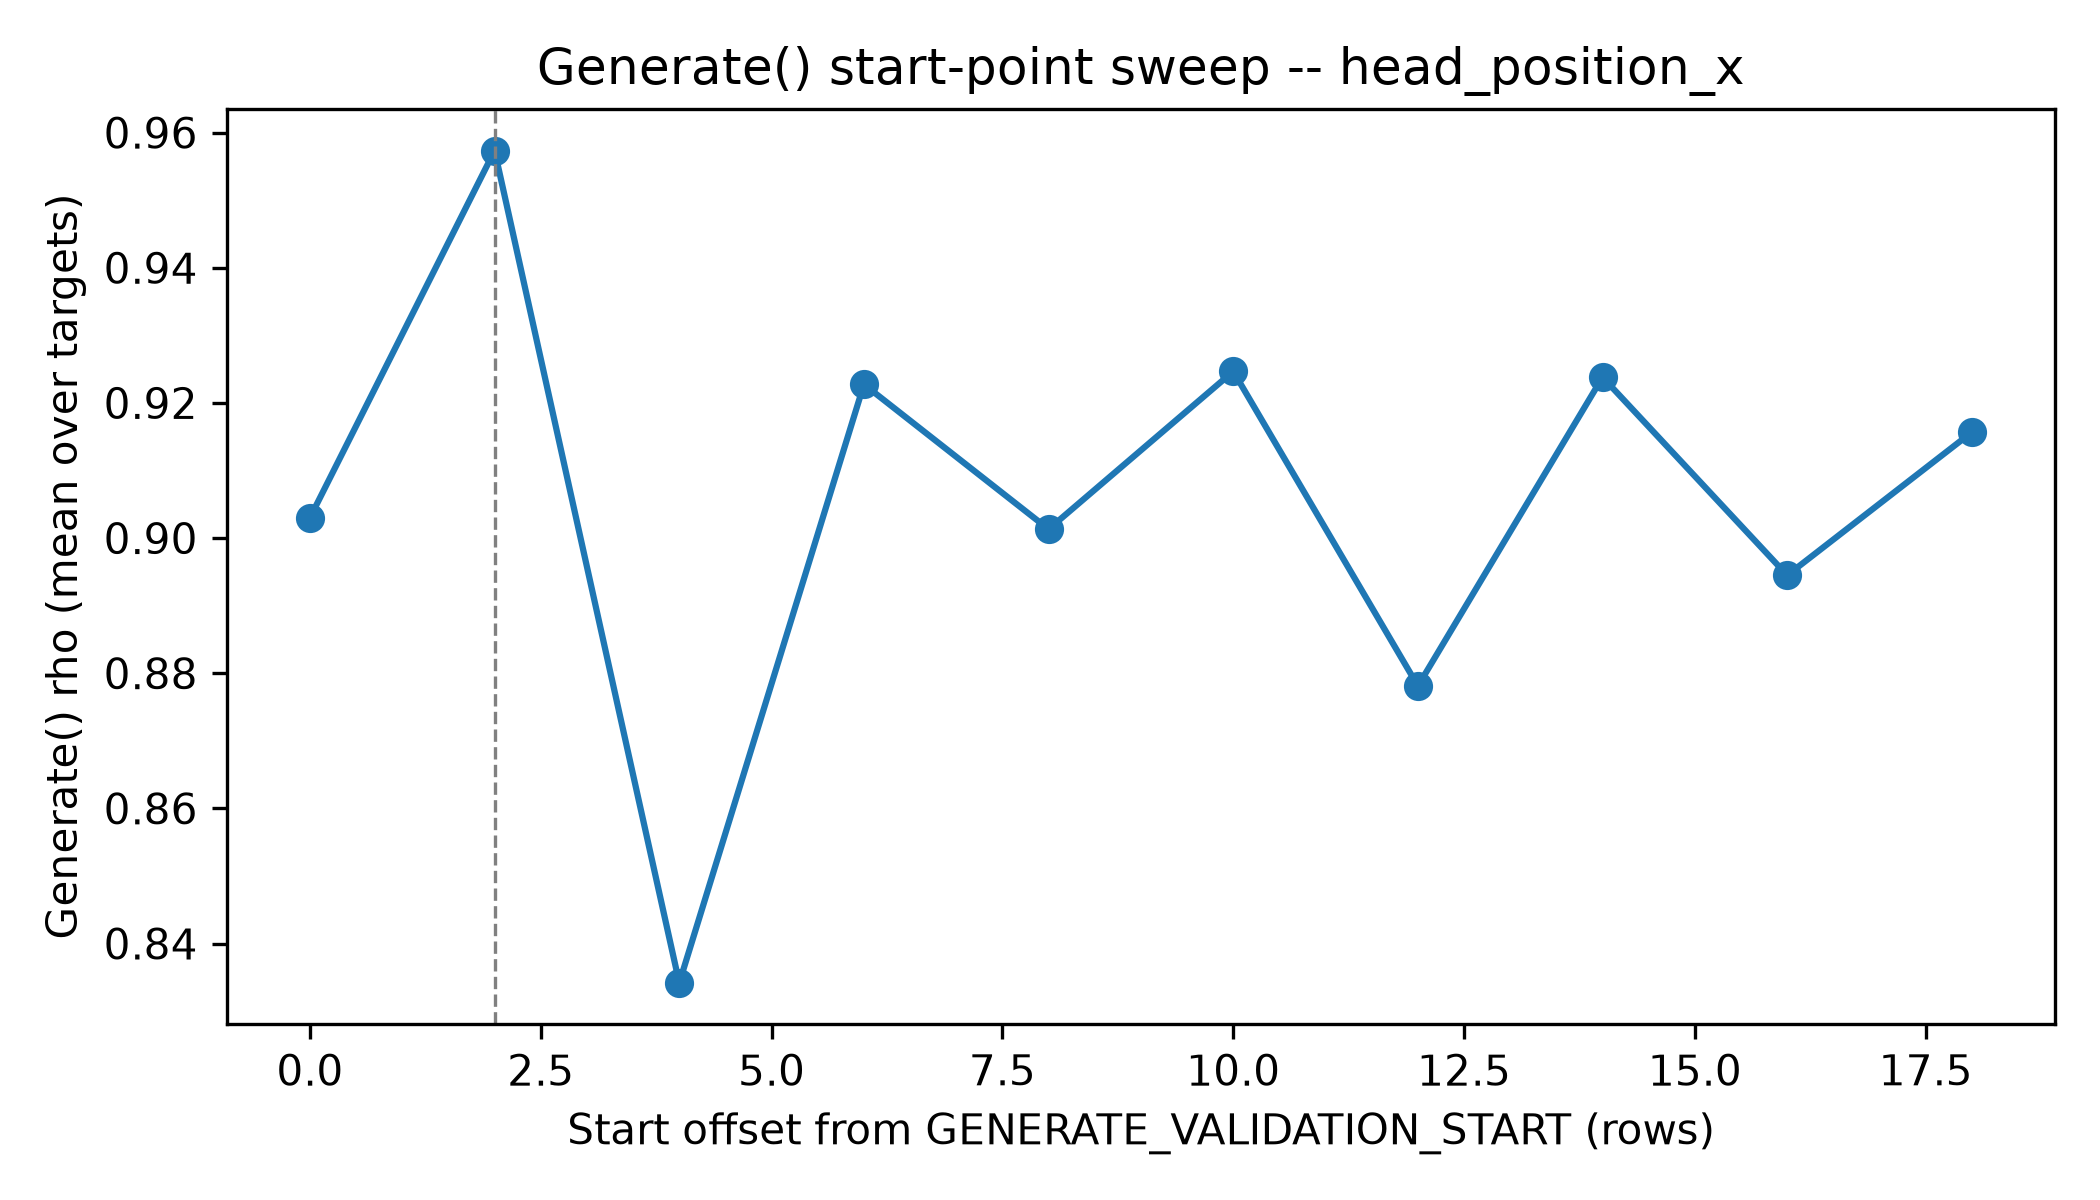
\includegraphics[width=0.7\textwidth]{figures/generate_start_sweep_head_position_x.png}
\caption{Real \texttt{sweep\_generate\_start()} output: mean Generate() rho across a range of candidate start rows, offset from \texttt{GENERATE\_VALIDATION\_START}. The swing from $\rho\approx0.83$ to $\rho\approx0.96$ across offsets 0--18 is a direct, real demonstration of exactly the sensitivity Section~\ref{sec:search} describes -- the same embedding and theta, scored very differently depending purely on which row the recursive simulation launches from.}
\label{fig:start-sweep}
\end{figure}

\subsection{Generate() vs.\ Forecast() vs.\ real data}
\begin{figure}[H]
\centering
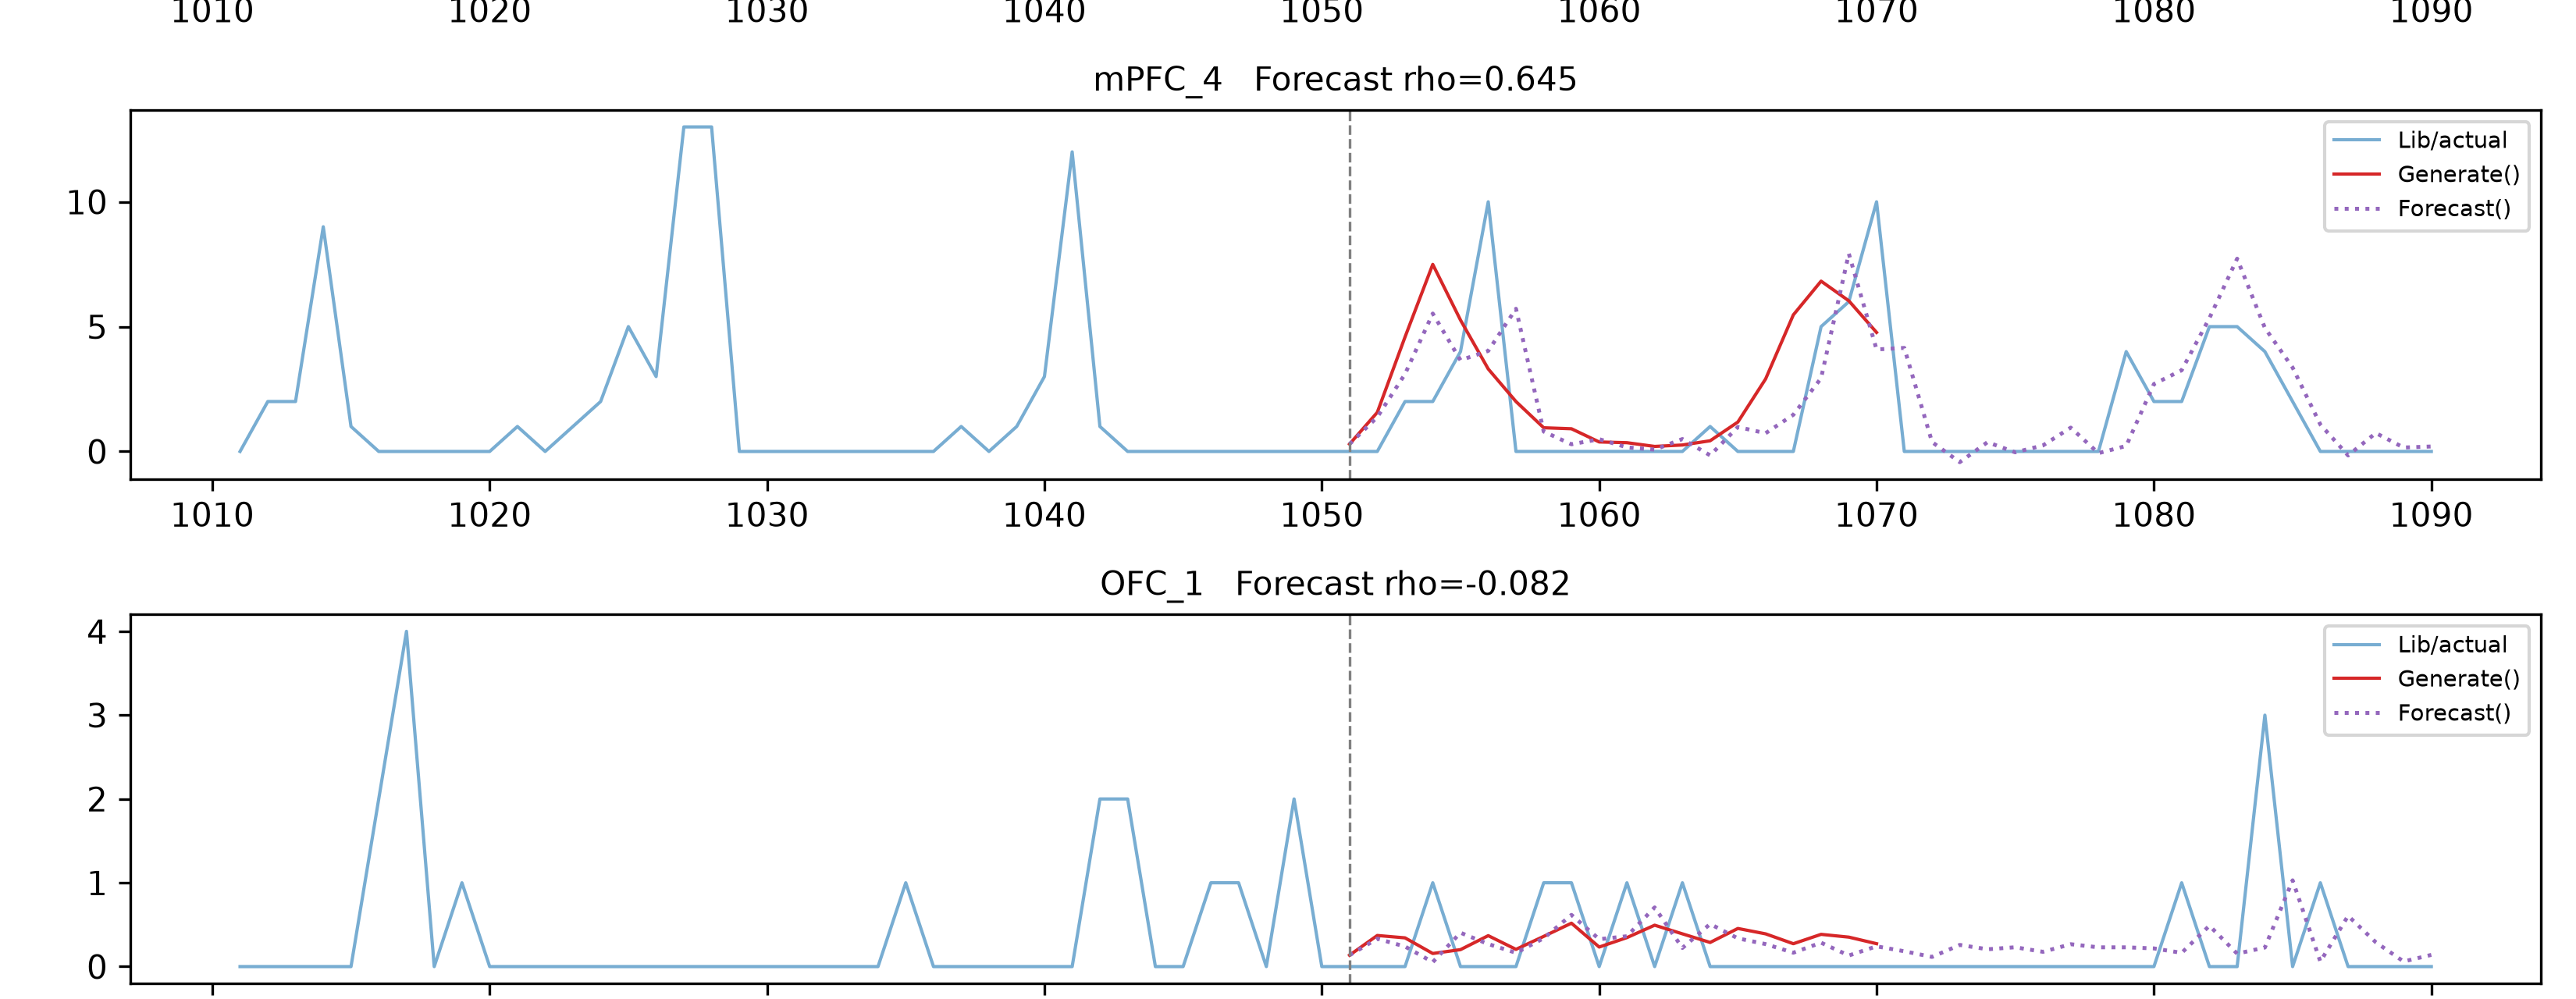
\includegraphics[width=0.92\textwidth]{figures/generate_forecast_crop.png}
\caption{Real \texttt{run\_forecast\_diagnostic()} output (cropped to 2 of the network's 46 node panels). mPFC\_4 (Forecast $\rho=0.645$) shows Generate() (solid red) and Forecast() (dotted purple) both tracking the real data's (blue) major peaks reasonably well through the held-out window; OFC\_1 (Forecast $\rho=-0.082$) shows both essentially failing to track a sparser, noisier real signal -- the per-node spread Section~\ref{sec:validation} exists to surface.}
\label{fig:generate-forecast}
\end{figure}

\subsection{MDE vs.\ unsupervised baselines (\texttt{run\_mde\_evaluate})}
\begin{center}
\begin{tabular}{lrrrr}
\toprule
Method & CAE & RMSE & R & $R^2$ \\
\midrule
\multicolumn{5}{l}{\textit{head\_position\_x}} \\
MDE  & 1961.86 & 20.581 & \textbf{0.570} & \textbf{0.325} \\
PCA  & 2259.15 & 23.727 & 0.220 & 0.048 \\
dMap & 2207.74 & 24.467 & $-$0.060 & 0.004 \\
\multicolumn{5}{l}{\textit{head\_position\_y}} \\
MDE  & 3860.56 & 43.388 & 0.370 & 0.137 \\
PCA  & 1772.23 & 19.312 & \textbf{0.747} & \textbf{0.558} \\
dMap & 1672.56 & 18.151 & \textbf{0.781} & \textbf{0.610} \\
\bottomrule
\end{tabular}
\end{center}
\pitfallbox{An honest, unfavorable-to-MDE result, reported rather than omitted:}{At this tiny channel cap, MDE's own selection beats both unsupervised baselines for \texttt{head\_position\_x} but loses to \emph{both} for \texttt{head\_position\_y} -- PCA and diffusion-map reconstructions score $R^2$ 4--5$\times$ higher. This is exactly the kind of result Section~\ref{sec:diagnostics}'s comparison exists to surface, and exactly why the sibling pipeline dropping this diagnostic (its Section~6) is a real loss of visibility, not a neutral simplification. Whether this reverses at full channel count/MDE\_D is an open, empirical question -- Section~\ref{sec:future}.}

\newpage
% =====================================================================
\section{Development History: Challenges, Investigations, and Design Decisions}
\label{sec:history}
% =====================================================================
Written for a reviewer, not a user: for every major issue, the observed symptom, what was actually wrong, the decision made, and the risk that decision leaves open.

\subsection{The nested-multiprocessing-pool blowup}
\label{sec:history-pool}
\textbf{Symptom:} jobs ran roughly two days regardless of dataset size, mode, or parameter choice. \textbf{Investigation:} process counts observed empirically (dozens of live processes from a single-digit core request); reading \texttt{pyEDM}'s installed source directly showed \texttt{CCM()} spawns a brand-new multiprocessing pool sized to the full visible core count on \emph{every single call} -- and this pipeline calls it once per channel pair or MDE candidate, tens of thousands of times, each paying a full spawn-and-reimport cost for 4--8 tiny KD-tree tasks. \textbf{Decision:} \texttt{\_sequential\_ccm\_workers}/\texttt{\_sequential\_ccm\_api} force every \texttt{CCM()} call in this process onto its sequential in-process path (Section~\ref{sec:dimx}), later reapplied inside every \texttt{ProcessPoolExecutor} worker via \texttt{\_mde\_wave\_worker\_init} once the wave-pool architecture (Stages 1--2) made that necessary. \textbf{Risk carried forward:} this patch must be manually kept in sync with the sibling pipeline (Section~\ref{sec:sibling}) -- it is duplicated code, not shared.

\subsection{A crash caught only by preserving the failing run's own data}
\textbf{Symptom:} the constructed network repeatedly came out empty or with no real driver edges. \textbf{Investigation:} rather than guess, a failed run's own interaction-matrix CSV was preserved and inspected directly -- it showed cells at \emph{exactly} 0.0, not small or negative, which a real correlation computation does not produce by chance. The convergence gate's "small" library size was a fixed percentage of the \emph{entire} dataset -- already well past where a real, low-dimensional relationship's cross-map skill saturates, so the gate was never shown a library size small enough to see a real relationship still improving. \textbf{Decision:} this diagnosis (and the resulting library-size recalibration) originates in the sibling pipeline's own development history (\texttt{docs/tsls-mde-gmn-pipeline.pdf}, "The empty-network investigation"); this pipeline's own nested-MDE design sidesteps the interaction-matrix path entirely for \texttt{MODE='MDE-GMN'} (Section~\ref{sec:stage1}), but \texttt{MODE='GMN'}'s CCM-based fallback path still depends on the same calibration.

\subsection{PCA crashing on delay-expansion warm-up rows}
\textbf{Symptom:} \texttt{run\_mde\_evaluate()} (Section~\ref{sec:diagnostics}) died late in a run -- roughly 23 hours in -- with an error from scikit-learn's PCA fit, which has zero \texttt{NaN} tolerance. \textbf{Investigation:} \texttt{expand\_delay\_columns()} shifts each observable forward by $|{\rm delay}|$ rows, leaving that many leading rows \texttt{NaN} (nothing precedes the start of the recording to shift in) -- these were reaching \texttt{mde\_df}'s library slice before PCA's fit. \textbf{Decision:} \texttt{run\_mde\_for\_target()} now computes \texttt{warmup = max(|d| for d in delay\_set)} and starts \texttt{lib} at \texttt{warmup+1} rather than row 1, so every delay column is fully populated for the entire library range before any downstream consumer (PCA included) sees it. \textbf{Risk carried forward:} this was found by a late, expensive crash, not by inspection -- any future new consumer of \texttt{mde\_df} that assumes zero \texttt{NaN} without checking this same warm-up convention could reintroduce an equivalent failure elsewhere in the pipeline.

\subsection{The all-NaN crash and the exception-guarding it motivated}
\label{sec:history-crash}
\textbf{Symptom:} job 37946756 (\texttt{MDE\_D=999}, effectively uncapped forward selection) got through its depth-0 seed with individual nodes already selecting 200--300+ drivers each, then failed 1 day 11 hours in, partway through the very first depth-1 wave. \textbf{Investigation:} the traceback led to \texttt{dimx/Run.py:161} -- \texttt{EDimDF['rho'].round(4).argmax()} -- raising \texttt{ValueError: Encountered all NA values} when a candidate's rho column was entirely \texttt{NaN}, a real failure mode inside third-party code this pipeline's own gates don't control. This propagated straight out of the wave's \texttt{ProcessPoolExecutor}, killing every other already-completed node's work in that wave alongside it. \textbf{Decision:} \texttt{\_failed\_mde\_result()} -- shaped identically to a legitimate zero-driver selection, so it dead-ends cleanly through the exact same downstream code path -- is now substituted at all three call sites that can hit this (Stage 1's wave loop, Stage 2's wave loop, and \texttt{main()}'s own depth-0 seed, added proactively once the first two fixes made clear the seed has the identical vulnerability one level up). \textbf{Separately}, \texttt{MDE\_D} was reduced from 999 to 30 for the time being: \texttt{CrossMapColumns}' own per-step ranking cost grows with how many columns are already selected, so a node selecting hundreds of drivers isn't just slower per candidate, it calls \texttt{CrossMapColumns} hundreds of times at steadily growing dimension -- the true root cause of the pathological wall-clock, not just the eventual crash. \textbf{Risk carried forward:} 999 remains the eventual target once this cost is properly characterized at intermediate \texttt{MDE\_D} values -- Section~\ref{sec:future}.

\subsection{Editing a shared, non-frozen script under a queued job}
\label{sec:history-shared-script}
\textbf{Symptom:} job 38857309 -- resubmitted specifically to pick up the exception-guarding fix above plus \texttt{MDE\_D=30} -- sat \texttt{PENDING} for roughly an hour, then \texttt{FAILED} 5 seconds after it finally started. \textbf{Investigation:} \texttt{sbatch} freezes the top-level submitted script's own content at submission time (confirmed via \texttt{scontrol show job}'s \texttt{Command=} field), but a script it calls by path -- \texttt{generate\_job\_description.sh} -- is read fresh off disk at run time, not frozen. That shared script's call signature was changed (an unused \texttt{<out\_dir>} argument dropped, Section~\ref{sec:storage}'s empty-directory fix) \emph{while this job was still queued}, so its still-old 5-argument call hit the new script's 4-argument usage error and the whole job aborted under \texttt{set -euo pipefail}. \textbf{Decision:} resubmitted once both sides were consistent; no code change resulted from this incident beyond awareness. \textbf{Risk carried forward:} any future edit to a shared, path-called script (as opposed to the top-level sbatch script itself) can break a job that is already queued but hasn't started -- there is no mechanism currently checking for this before making such an edit.

\subsection{Resource sizing: from evidence-free headroom to measured right-sizing}
\label{sec:history-resources}
\textbf{Symptom:} \texttt{--cpus-per-task}/\texttt{--mem} were raised over several iterations (32$\to$128 cores, 48G$\to$200G$\to$500G) chasing OOM kills and timeouts (job 36515744 OOM'd at $\approx$49.75G against a 48G request; job 36969664 timed out at 3 days with \texttt{MaxRSS}$\approx$197G against a 200G request) -- each raise was real headroom against a real measured failure, but by 128 cores/500G the request was simply this partition's own stated ceiling, not a number derived from an actual usage model at the current \texttt{MDE\_D=30} scale. \textbf{Investigation:} once job 38870714 sat queued as the \emph{only} pending job on the entire compute partition, \texttt{sinfo} showed why: 128 cores + 500G is a whole node, and at that moment zero of the partition's 128-core nodes were fully idle, while 64 cores + 300G already fit on 23 currently-partially-allocated nodes (this partition shares nodes between jobs). Cross-checked against real \texttt{MaxRSS}/\texttt{TotalCPU} data: the one full run that completed cleanly (job 36786285, pre-two-stage) peaked at $\approx$58G RSS on 32 cores; even the \texttt{MDE\_D=999} pathological run (job 37946756, Section~\ref{sec:history-crash}) peaked at only $\approx$135G and averaged just $\approx$57 of its 128 allocated cores actually busy. \textbf{Decision:} reduced to \texttt{--cpus-per-task=64}, \texttt{--mem=300G} -- real headroom above every measured number, not a tight fit, while fitting far more of the partition's actual currently-free capacity. \textbf{Risk carried forward:} no run has yet completed at exactly \texttt{MDE\_D=30}/\texttt{REGION\_CHANNEL\_CAP=999} to confirm this sizing against; if a run at this configuration is OOM-killed or shows every core saturated, raise both back toward the partition ceiling.

\subsection{The \texttt{CA1\_22} crash: two fixes made together}
\label{sec:history-prefilter-order}
\textbf{Symptom:} job 39605472 crashed 1m20s in with \texttt{ValueError: invalid literal for int() with base 10: 'CA1\_22'}.\\
\textbf{Investigation:} the traceback led to \texttt{observable\_and\_delay()} $\to$ \texttt{\_parse\_delayed\_column\_name()}, which assumes any column name not found verbatim in \texttt{raw\_columns} must carry a \texttt{::delay-N} suffix to strip and parse -- but \texttt{CA1\_22} carried no such suffix; it was simply absent from \texttt{raw\_columns}. A log excerpt pinned the exact moment: \texttt{"CCM pre-filter: kept 36/90 observables (rho >= 0.2) for ['head\_position\_x']"} printed successfully, then the very next step -- Stage 1's own \texttt{build\_nested\_mde\_network()}, processing \texttt{head\_position\_x}'s depth-0 result -- crashed on \texttt{CA1\_22}: a real driver MDE had selected against the full 90-observable pool in \texttt{main()}, before the CCM pre-filter (Section~\ref{sec:ccm-prefilter}) narrowed the 36-observable pool Stage 1 itself searches (Section~\ref{sec:why-depth0-explicit}'s Figure~\ref{fig:prefilter-ordering} illustrates the mismatch directly). The sibling pipeline hit the identical bug the same way, on its own \texttt{\_tsls}-suffixed column names -- job 39605473 crashed on \texttt{'CA1\_12\_tsls'} (sibling document, "The \texttt{CA1\_12\_tsls} crash: two fixes made together"). A first patch, verified via resubmission (job 39655803), added a marker-presence fallback to \texttt{observable\_and\_delay()} so an unrecognized name is treated as a plain delay-0 observable rather than crashing -- this kept jobs running, but review found it papered over the mismatch rather than fixing it, alongside a second, unrelated design gap: Stage 2's own real-observable picks never recursed (Section~\ref{sec:stage2-recursion}).\\
\textbf{Decision (per explicit request, both fixes made together):} (1) \texttt{main()} now runs \texttt{ccm\_prefilter\_observables()} once per target group \emph{before} seeding depth-0, so depth-0 and every later nested-MDE round search the exact same filtered pool -- the mismatch this crash depended on can no longer occur on a normal run. (2) Stage 1 and Stage 2 were unified into one per-wave BFS (Section~\ref{sec:stage1}) so a Stage-2 real-observable pick recurses exactly like a Stage-1 one. Both were verified on real data locally (isolated probe calls confirmed Stage-2-style real-observable picks actually recurse, on both this pipeline's 1\,Hz data and the sibling pipeline's 40\,Hz data) before the next cluster submission (job 39670999).\\
\textbf{Risk carried forward:} the \texttt{observable\_and\_delay()} fallback was kept, not removed -- it is now a pure safety net for cross-job cache reuse (\texttt{REUSE\_BEST\_PARAMS}), where a reused \texttt{mde\_results} entry can legitimately come from an earlier job that used a different \texttt{CCM\_PREFILTER\_RHO\_MIN}/\texttt{CCM\_PREFILTER\_E}, or predates the pre-filter feature entirely, and so can still reference an observable absent from \emph{this} run's own filtered \texttt{raw\_columns}. A reviewer should not read its continued presence as evidence the ordering bug is still live on a normal (non-cache-reuse) run.

\newpage
% =====================================================================
\section{Known Limitations and Open Questions}
\label{sec:limitations}
% =====================================================================
\begin{itemize}
  \item \textbf{No TSLS (or equivalent) conversion of raw spike counts.} Section~\ref{sec:sibling} states this as a fact; it is worth restating here as an open question. The sibling pipeline's own stated rationale for TSLS -- that Takens embedding needs local geometry a sparse, mostly-zero spike train doesn't have -- was never evaluated against this pipeline's raw, 1 Hz-binned counts (mean $\approx$0.12/bin, the overwhelming majority exactly 0). Whether that sparsity meaningfully degrades this pipeline's own embeddings, or whether coarser 1 Hz binning already provides enough local structure for Simplex/S-map/CCM to work with, has not been directly tested here the way the sibling pipeline's TSLS-vs-raw question was.
  \item \textbf{MDE forward-selection is single-threaded within one call} (\texttt{dimx.MDE} itself, Section~\ref{sec:dimx}) -- this pipeline's own wave-level parallelism (Sections~\ref{sec:stage1}--\ref{sec:stage2}) parallelizes \emph{across} nodes, but one node's own forward-selection loop over its candidate pool is not itself parallel, the same regression the sibling pipeline's \texttt{proper\_mde} port also carries.
  \item \textbf{Theta retuning has no TSLS-aware path} (Section~\ref{sec:search}) -- moot for correctness here specifically because this pipeline never TSLS-converts in the first place, but worth remembering if that changes.
  \item \textbf{Backbone topology construction is order-dependent, not globally optimal} (Section~\ref{sec:stage1}) -- which edges survive when a cycle is possible depends on BFS traversal order (wave order, then per-node selection order), not a global optimization over which edge set maximizes total network strength while staying acyclic.
  \item \textbf{Try/except-guarded loops can hide programming bugs, not just expected failures} (Sections~\ref{sec:history-crash}, \ref{sec:search}) -- deliberate (one bad node/candidate should not abort an entire wave or search), but any future addition to a guarded loop should be checked in isolation before assuming a silent failure means "no signal here."
  \item \textbf{No run has yet completed at the intended full scale} (\texttt{MDE\_D=30}, \texttt{REGION\_CHANNEL\_CAP=999}) under the current two-stage design -- every genuinely completed run documented here (Section~\ref{sec:outputs}) is at a much smaller channel cap. The MDE-vs-baseline result in Section~\ref{sec:outputs} in particular should not be assumed to hold at full scale.
\end{itemize}

\newpage
% =====================================================================
\section{Future Directions}
\label{sec:future}
% =====================================================================
Concrete next steps, several of them direct consequences of what this document's own research (Sections~\ref{sec:outputs}, \ref{sec:history-resources}) actually found rather than speculative wishlist items.

\begin{enumerate}[leftmargin=1.4em]
  \item \textbf{Validate the full-scale run once it completes.} Job 38871293 (\texttt{MDE\_D=30}, \texttt{REGION\_CHANNEL\_CAP=999}, 64 cores/300G) is the first attempt at this exact two-stage design at anything near full scale. Once it finishes, re-run this document's Section~\ref{sec:outputs} analysis against its real output -- network size/edge count, fidelity distribution, and the MDE-vs-PCA-vs-diffusion-map comparison in particular, since Section~\ref{sec:outputs}'s small-scale result was unfavorable to MDE for one of the two targets.
  \item \textbf{Characterize the true MDE\_D-vs-cost curve.} Section~\ref{sec:history-crash} established that \texttt{MDE\_D=999} is pathological and \texttt{MDE\_D=30} is untested at full scale; a systematic sweep at a few intermediate values (e.g.\ 30, 60, 120, 250) against \texttt{REGION\_CHANNEL\_CAP=999} would turn "999 is the eventual target" from an aspiration into a scheduled, evidence-based increase.
  \item \textbf{Re-check resource sizing against a completed full-scale run.} Section~\ref{sec:history-resources}'s 64-core/300G sizing is grounded in the best data available at the time (a pre-two-stage completed run and a pathological, uncompleted \texttt{MDE\_D=999} run) -- neither is the configuration actually running now. Once job 38871293 (or its successor) completes, its own \texttt{MaxRSS}/core-utilization should directly confirm or correct this sizing.
  \item \textbf{Investigate the raw-spike-count-vs-TSLS question directly}, the way the sibling pipeline's own noCCM investigation (\texttt{docs/tsls-mde-gmn-pipeline.pdf}, "Removing a validation gate versus recalibrating it") tested a real hypothesis on real data rather than arguing from first principles: run a handful of specific, currently-selected drivers through MDE/CCM on both the raw counts and a TSLS-converted version of the same channels, and compare selection stability and cross-map skill directly.
  \item \textbf{Explore \texttt{STAGE2\_ALLOW\_REAL\_OBSERVABLES=true}} as a genuine algorithmic variant, not just a currently-off toggle: does letting Stage 2 introduce real observables Stage 1 never reached change which nodes end up in the network, and does it change fidelity for better or worse.
  \item \textbf{Parallelize \texttt{dimx.MDE}'s own forward-selection loop} (Section~\ref{sec:limitations}) -- the single largest remaining performance gap this document's own resource-history section (Section~\ref{sec:history-resources}) did not touch, since it targets between-node parallelism, not within-node.
  \item \textbf{Extend the exception-guarding pattern's own test coverage} -- Section~\ref{sec:history-crash}'s fix was verified with a standalone smoke test of \texttt{\_failed\_mde\_result()}'s shape, but not yet against a real, deliberately-triggered failure inside a live \texttt{ProcessPoolExecutor} wave at scale.
  \item \textbf{Confirm a real crash-and-resume cycle end-to-end.} The cross-job cache architecture (Section~\ref{sec:reuse}) is designed to let a resubmission pick up node-by-node after a timeout or crash; this has not yet been directly demonstrated on a real job pair (kill one job partway through a wave, resubmit identically, confirm the resumed job's log shows cache hits for already-completed nodes and fresh computation only for the rest).
\end{enumerate}

\newpage
% =====================================================================
\section*{Appendix A: Configuration Parameter Reference}
\addcontentsline{toc}{section}{Appendix A: Configuration Parameter Reference}
% =====================================================================
\begin{longtable}{@{}>{\raggedright\arraybackslash}p{4.0cm}>{\raggedright\arraybackslash\small}p{2.6cm}>{\raggedright\arraybackslash}p{7.9cm}@{}}
\toprule
\textbf{Parameter} & \textbf{Default} & \textbf{Meaning} \\
\midrule
\endhead
\texttt{DATA_FILE} & 4\,Hz CSV & Raw, per-region-binned spike-count + behavior recording (current runs use the 1\,Hz file). \\
\texttt{MODE} & \texttt{MDE-GMN} & \texttt{MDE-GMN} runs the two-stage nested-MDE design (Sections~\ref{sec:stage1}--\ref{sec:stage2}); \texttt{GMN} uses the original CCM interaction-matrix path instead. \\
\texttt{GMN_MODE} & \texttt{combined} & One shared network for all targets vs.\ \texttt{separate} (one network per target). \\
\texttt{TARGETS} & position x/y & Behavioral columns to predict. \\
\texttt{LIB_RATIO} & 0.5 & Fraction of rows forming the MDE library segment $[0,A)$ (Section~\ref{sec:split}). \\
\texttt{MDE_VALIDATION_RATIO} & 0.5 & Fraction of the post-library remainder given to $[A,B)$ vs.\ $[B,\mathrm{end})$. \\
\texttt{GENERATE_LENGTH} & 0 (full) & Steps per \texttt{Generate()} call; clamped to \texttt{GENERATE\_VALIDATION\_LENGTH} (Section~\ref{sec:split}'s pitfall box). \\
\texttt{MDE_D} & 20 & Max real observables MDE may select per round, per stage/nesting level. \\
\texttt{TP} & 1 & Prediction interval every MDE ranking/validation call uses (Section~\ref{sec:dimx}). \\
\texttt{EMBED_DIM_RHO_MIN} / \texttt{CROSS_MAP_RHO_MIN} & 0.2 / 0.2 & MDE's own embedding-dimension / ranking-stage acceptance thresholds. \\
\texttt{CCM_PREFILTER_RHO_MIN} & 0.2 & CCM pre-filter rho cutoff (Section~\ref{sec:ccm-prefilter}); 0 disables the filter, pool passes through unchanged. \\
\texttt{CCM_PREFILTER_E} & 3 & Static embedding dimension for the pre-filter's own CCM calls -- no per-candidate auto-select (would defeat the point of a \emph{cheap} filter); default matches the sibling pipeline's own \texttt{MULTI\_MDE\_E} default for cross-pipeline consistency, even though this pipeline has no \texttt{multi\_proper\_mde}-style joint-MDE concept of its own. Deliberately different from the sibling pipeline's own \texttt{CCM\_PREFILTER\_E} default of 7 (1\,Hz raw counts here vs.\ 40\,Hz TSLS data there, at the same \texttt{tau=-1}). \\
\texttt{LIBSIZE_RATIOS} & 0.05,0.10,0.20,0.40,0.6,0.8,0.9 & Library-size sweep for the CCM pre-filter, as fractions of \texttt{PREDICTION\_START}. \\
\texttt{EXCLUSION_RADIUS} & \texttt{auto} & Dynamic per-call Theiler window (Section~\ref{sec:exclusion-radius}) vs.\ a fixed integer. \\
\texttt{NESTED_M} & 1 & Additional nested-MDE rounds beyond depth 0; 0 = uncapped (Section~\ref{sec:stage1}). \\
\texttt{STAGE2_ALLOW_REAL_OBSERVABLES} & false & Whether Stage 2 may introduce a real observable Stage 1 never reached (Section~\ref{sec:stage2}). \\
\texttt{REGION_CHANNEL_CAP} & 999 & First $N$ channels per region offered as candidates (999 $\approx$ uncapped, 468 real observables in the current dataset). \\
\texttt{DELAY_SOURCE} & \texttt{lag_mode} & \texttt{lag_mode} (auto-derived) vs.\ \texttt{explicit} (\texttt{DELAY\_SET} list). \\
\texttt{LAG_MODE} & \texttt{generation_length_adjusted} & Bound on Stage 2's deepest lag: tied to \texttt{GENERATE\_LENGTH} vs.\ \texttt{every_lag_possible}. \\
\texttt{LAG_DENSITY} / \texttt{LAG_STEP} & \texttt{strided} / 5 & Sampling density of the lag bound; \texttt{LAG\_STEP=1} forced in current runs (Section~\ref{sec:stage2}). \\
\texttt{GENERATE_START_MIN/MAX/STEP_OFFSET} & 0/1/50 & Candidate \texttt{Generate()} start-row offsets from $B$ (Section~\ref{sec:search}). \\
\texttt{THETA_RANGE} & 15 values & S-map localization search grid (Section~\ref{sec:search}). \\
\texttt{E_RANGE} / \texttt{TAU_RANGE} & 3--15 / $-$15--0 & \texttt{MODE='GMN'} only -- CCM interaction-matrix grid search. \\
\texttt{RUN_MDE_DIAGNOSTICS} & true & Toggles Section~\ref{sec:diagnostics}. \\
\texttt{REUSE_BEST_PARAMS} & false & Enables the cross-job fingerprinted cache (Section~\ref{sec:reuse}). \\
\bottomrule
\end{longtable}

\newpage
% =====================================================================
\section*{Appendix B: Glossary}
\addcontentsline{toc}{section}{Appendix B: Glossary}
% =====================================================================
\begin{description}[leftmargin=3.2cm, style=nextline]
  \item[MDE] Manifold Dimension eXpansion -- greedy, causality-gated forward selection (Section~\ref{sec:dimx}). This pipeline uses \texttt{dimx.MDE} directly (unlike the sibling pipeline's \texttt{proper\_mde}).
  \item[CCM pre-filter] \texttt{ccm\_prefilter\_observables()} (Section~\ref{sec:ccm-prefilter}) -- a cheap, once-per-target-group CCM(observable $\to$ target) relevance screen run before depth-0, shrinking the candidate pool every later nested-MDE round also searches.
  \item[Stage 1 / Stage 2] This pipeline's own two-stage nested-MDE network construction (Sections~\ref{sec:stage1}--\ref{sec:stage2}) -- no notebook precedent.
  \item[GMN] Generative Manifold Network -- the directed graph this pipeline builds and simulates (Sections~\ref{sec:stage1}--\ref{sec:smap}).
  \item[Generalized embedding] A per-driver, per-delay embedding built directly from the discovered graph (Section~\ref{sec:smap}), replacing gmn's own shared, uniform $(E,\tau)$.
  \item[CCM] Convergent Cross Mapping -- the causality test inside MDE's own gate (Section~\ref{sec:dimx}).
  \item[S-map] Sequential locally weighted global linear maps -- the local-regression engine every node uses (Section~\ref{sec:smap}).
  \item[$\theta$] S-map's localization parameter -- the only quantity this pipeline still grid-searches (Section~\ref{sec:search}).
  \item[Three-way split] $[0,A)$/$[A,B)$/$[B,\mathrm{end})$ -- MDE library / MDE validation / Generate-Forecast validation (Section~\ref{sec:split}).
  \item[Fingerprint] A hash of every input that determines one cacheable stage's outcome, used to safely skip recomputation across job resubmissions (Section~\ref{sec:reuse}).
\end{description}

\end{document}
